\subsection{Test di integrazione}
Questa tipologia di test serve per verificare che le varie componenti del sistema interagiscono tra loro nella maniera attesa. La strategia per definire -e poi eseguire- i seguenti test, è quella di partire dalle singole componenti per poi realizzare le varie funzionalità incrementalmente durante lo sviluppo del prodotto finale. Questo potrà essere di aiuto in caso di errori, in quanto essi si presenteranno in un ambiente già testato e funzionante. \\
Per ogni test viene specificato il suo codice univoco, la descrizione e lo stato di implementazione attuale.

	\begin{longtable}{|>{\centering\arraybackslash}m{1.6cm}|>{\centering\arraybackslash}m{6.41cm}|>{\centering\arraybackslash}m{3.1cm}|}		
		\rowcolor{LightBlue}
		\textbf{\textcolor{white}{Test}}
		& \multicolumn{1}{|c|}{\textbf{\textcolor{white}{ Descrizione}}}\\
		\hline
		TI1
		& Test d’integrazione front-end e back-end per la corretta visualizzazione del front-end.
		\\ \hline
		\rowcolor{LightGray}
		TI2
		& Test d’integrazione front-end e back-end per l'invio dei dati al front-end.
		\\ \hline
		TI3
		& Test d’integrazione front-end e back-end per la ricezione di dati dal front-end tramite POST.
		\\ \hline
		\rowcolor{LightGray}
		TI4
		& Test d’integrazione front-end e back-end per la ricezione di dati dal front-end tramite GET.
		\\ \hline
		TI5
		& Test d’integrazione tra back-end e Hunpos per il POS-Tagging$^*$.
		\\ \hline
		\rowcolor{LightGray}
		TI6
		& Test d’integrazione tra back-end e Hunpos per il training.
		\\ \hline	
		TI7
		& Test d’integrazione tra back-end e Google Firebase Realtime Database per la lettura dalla base di dati.
		\\ \hline	
		\rowcolor{LightGray}
		TI8
		& Test d’integrazione tra back-end e Google Firebase Realtime Database per la scrittura sulla base di dati.
		\\ \hline	
		TI9
		& Test d’integrazione tra back-end e Google Firebase Realtime Database per la modifica della base di dati.
		\\ \hline	
		\rowcolor{LightGray}
		TI10
		& Test d’integrazione tra back-end e Google Firebase Realtime Database per l'eliminazione dalla base di dati.
		\\ \hline	
		\caption{Test di integrazione - descrizione}
\end{longtable}


\subsection{Test di unità}
\begin{longtable}{|>{\centering\arraybackslash}m{1.6cm}|>{\centering\arraybackslash}m{6.41cm}|>{\centering\arraybackslash}m{3.1cm}| c |}		
		\rowcolor{LightBlue}
		\textbf{\textcolor{white}{Test}}
		& \multicolumn{1}{|c|}{\textbf{\textcolor{white}{ Descrizione}}}\\
		\hline
		TU & Verifica che il metodo ritorni l'id corretto della classe su cui è richiamato. \\ \hline
		TU & Verifica che il metodo ritorni il nome corretto della classe su cui è richiamato. \\ \hline
		TU & Verifica che il metodo ritorni la descrizione corretta della classe su cui è richiamato.\\ \hline
		TU & Verifica che venga ritornato l'id corretto dell'insegnante creatore della classe su cui il metodo è richiamato. \\ \hline
		TU & Verifica che venga ritornata la corretta lista di studenti appartenenti alla classe su cui il metodo è richiamato.  \\ \hline
		TU & Verifica che venga ritornata la corretta lista di esercizi assegnati alla classe su cui il metodo è richiamato.\\ \hline
		TU & Verifica che ritorni il giusto numero di studenti studenti appartenenti alla classe su cui il metodo è richiamato.  \\ \hline
		TU & Verifica che il metodo elimini correttamente uno studente dalla lista di quelli appartenenti alla classe su cui è  richiamato.  \\ \hline
		TU & Verifica che il metodo elimini correttamente un esercizio dalla lista di quelli assegnati alla classe su cui è  richiamato.\\ \hline
		TU & Verifica che il metodo aggiunga correttamente uno studente dalla lista di quelli appartenenti alla classe su cui è  richiamato.\\ \hline
		TU & Verifica che il metodo aggiunga correttamente un esercizio dalla lista di quelli assegnati alla classe su cui è  richiamato. \\ \hline
		TU & Verifica che venga ritornato "true" se uno studente appartiene alla classe su cui il metodo viene richiamato; "false" altrimenti.  \\ \hline	
		TU & Verifica che il metodo riporti correttamente le informazioni relative ad una classe in formato JSON. \\ \hline	
		TU & Verifica che il metodo ritorni il valore della chiave dell'esercizio su cui è richiamato. \\ \hline
		TU & Verifica che venga ritornata la corretta frase dell'esercizio su cui il metodo è richiamato. \\ \hline
		TU & Verifica che il metodo ritorni un nuovo riferimento a POSManager.\\ \hline
		TU & Verifica che venga ritornato il corretto id dell'autore dell'esercizio su cui il metodo è richiamato.\\ \hline
		TU & Verifica che venga modificata correttamente la chiave dell'esercizio su cui il metodo è stato richiamato.\\ \hline
		TU & Verifica che venga modificata correttamente la frase dell'esercizio su cui il metodo è stato richiamato.\\ \hline
		TU & Verifica che venga modificata correttamente la soluzione dell'esercizio su cui il metodo è stato richiamato.\\ \hline
		TU & Verifica che venga aggiunta correttamente la soluzione alla lista delle soluzioni dell'esercizio su cui il metodo è stato richiamato.\\ \hline
		TU & Verifica che venga ritornata la corretta lista di soluzioni dell'esercizio su cui il metodo è richiamato.\\ \hline
		TU & Verifica che venga aggiunta correttamente una valutazione all'esercizio su cui il metodo è stato richiamato.\\ \hline
		TU & Verifica che venga ritornata la soluzione corrente dell'esercizio su cui il metodo è richiamato.\\ \hline
		TU & Verifica che venga ritornata la corretta soluzione automatica dell'esercizio su cui il metodo è richiamato. \\ \hline
		TU & Verifica che venga ritornata la frase splittata dell'esercizio su cui il metodo viene richiamato.\\ \hline
		TU & Verifica che venga inserita correttamente una valutazione alla soluzione corrente dell'esercizio su cui il metodo è richiamato.\\ \hline		
		TU & Verifica che il metodo riporti correttamente le informazioni relative ad un esercizio in formato JSON. \\ \hline	
		TU & Verifica che il metodo ritorni lo username corretto dello studente su cui è richiamato.\\ \hline
		TU & Verifica che il metodo ritorni il nome corretto dello studente su cui è richiamato.  \\ \hline
		TU & Verifica che il metodo ritorni il cognome corretto dello studente su cui è richiamato. \\ \hline
		TU & Verifica che il metodo ritorni la città corretta dello studente su cui è richiamato.\\ \hline
		TU & Verifica che il metodo ritorni la scuola corretta dello studente su cui è richiamato. \\ \hline
		TU & Verifica che il metodo ritorni la password corretta dello studente su cui è richiamato. \\ \hline
		TU & Verifica che il metodo ritorni "true" se vi è corrispondenza tra la prima e seconda password inserita dallo studente in fase di registrazione; "false" altrimenti.  \\ \hline
		TU & Verifica che il metodo ritorni l'id corretto dello studente su cui è richiamato.\\ \hline
		TU & Verifica che il metodo modifichi correttamente l'id dello studente su cui è richiamato. \\ \hline
		TU & Verifica che il metodo ritorni "false" se l'utente su cui è richiamato è uno studente, "true" se è un insegnante. \\ \hline
		TU & Verifica che il metodo ritorni "true" se l'utente su cui è richiamato è uno studente, "false" se è un insegnante. \\ \hline
		TU & Verifica che venga ritornata la corretta lista delle classi a cui appartiene lo studente su cui il metodo è richiamato.  \\ \hline
		TU & Verifica che il metodo ritorni la corretta media dello studente su cui è richiamato. \\ \hline
		TU & Verifica che il metodo ritorni lo username corretto dell'insegnante su cui è richiamato.\\ \hline
		TU & Verifica che il metodo ritorni il nome corretto dell'insegnante su cui è richiamato.  \\ \hline
		TU & Verifica che il metodo ritorni il cognome corretto dell'insegnante su cui è richiamato. \\ \hline
		TU & Verifica che il metodo ritorni la città corretta dell'insegnante su cui è richiamato.\\ \hline
		TU & Verifica che il metodo ritorni la scuola corretta dell'insegnante su cui è richiamato. \\ \hline
		TU & Verifica che il metodo ritorni la password corretta dell'insegnante su cui è richiamato. \\ \hline
		TU & Verifica che il metodo ritorni l'email corretta dell'insegnante su cui è richiamato. \\ \hline
		TU & Verifica che il metodo ritorni il codice INPS corretto dell'insegnante su cui è richiamato. \\ \hline
		TU & Verifica che il metodo ritorni "false" se l'utente su cui è richiamato è uno studente, "true" se è un insegnante. \\ \hline
		TU & Verifica che venga ritornata la corretta lista delle classi create dall'insegnante su cui il metodo è richiamato.  \\ \hline
		TU & Verifica che il metodo riporti correttamente le informazioni relative ad un insegnante in formato JSON. \\ \hline	
		TU & Verifica che il metodo ritorni il valore della chiave della soluzione su cui è richiamato.  \\ \hline
		TU & Verifica che il metodo ritorni l'id dell'autore della soluzione su cui è richiamato. \\ \hline
		TU & Verifica che il metodo ritorni gli argomenti della soluzione su cui è richiamato. \\ \hline
		TU & Verifica che il metodo ritorni la difficoltà della soluzione su cui è richiamato. \\ \hline
		TU & Verifica che il metodo ritorni "true" se la soluzione su cui è richiamato è pubblica; "false" altrimenti. \\ \hline
		TU & Verifica che il metodo modifichi lo stato di una soluzione da pubblico a privato o viceversa. \\ \hline
		TU & Verifica che il metodo ritorni i tag della soluzione su cui è richiamato. \\ \hline
		TU & Verifica che il metodo ritorni le valutazioni della soluzione su cui è richiamato. \\ \hline
		TU & Verifica che il metodo ritorni le valutazioni della soluzione su cui è richiamato in formato JSON.\\ \hline
		TU & Verifica che il metodo ritorni la data della soluzione su cui è richiamato \\ \hline
		TU & Verifica che il metodo aggiunga correttamente una valutazione alla soluzione su cui è richiamato\\ \hline
		TU & Verifica che il metodo ritorni una valutazione tra 0 e 10 della soluzione su cui è richiamato \\ \hline
		TU & Verifica che il metodo ritorni un'instanza di DbClassManager.  \\ \hline
		TU & Verifica che il metodo elimini correttamente una classe dal database.  \\ \hline
		TU & Verifica che il metodo elimini correttamente uno studente di una classe.  \\ \hline
		TU & Verifica che il metodo elimini correttamente un esercizio di una classe.  \\ \hline
		TU & Verifica che il metodo aggiunga correttamente uno studente di una classe.  \\ \hline
		TU & Verifica che il metodo aggiunga correttamente una classe al database. \\ \hline
		TU & Verifica che il metodo aggiunga correttamente un esercizio di una classe.  \\ \hline
		TU & Verifica che il metodo ritorni la corretta lista di studenti iscritti ad una classe.  \\ \hline
		TU & Verifica che il metodo ritorni la corretta lista di esercizi assegnati ad una classe.  \\ \hline
		TU & Verifica che il metodo ritorni la corretta lista di classi create da uno specifico insegnante.  \\ \hline
		TU & Verifica che il metodo ritorni correttamente le informazioni di una classe.  \\ \hline
		TU & Verifica che il metodo crei correttamente un'istanza di ClassClient.  \\ \hline
		TU & Verifica che il metodo crei correttamente un'istanza di UserClient.  \\ \hline
		TU & Verifica che il metodo crei correttamente un'istanza di ExerciseClient.  \\ \hline
		TU & Verifica che il metodo ritorni correttamente un'istanza di UserClient.  \\ \hline
		TU & Verifica che il metodo ritorni correttamente un'istanza di ClassClient  \\ \hline
		TU & Verifica che il metodo ritorni correttamente un'istanza di ExerciseClient.  \\ \hline
		TU & Verifica che ritorni la frase dell'esercizio su cui il metodo è richiamato correttamente splittata.  \\ \hline
		TU & Verifica che il metodo inserisca correttamente un esercizio nel database.  \\ \hline
		TU & Verfica che il metodo ricerchi correttamente un esercizio nel database.  \\ \hline
		TU & Verfica che il metodo ricerchi correttamente una soluzione nel database.  \\ \hline
		TU & Verifica che vengano ritornate la frase dell'esercizio su cui il metodo è richiamato.  \\ \hline
		TU & Verifica che vengano ritornate le informazioni dell'esercizio su cui il metodo è richiamato.  \\ \hline
		TU & Verifica che venga ritornata la media delle valutazioni delle soluzioni che gli studenti hanno fornito all'esercizio su cui il metodo è richiamato  \\ \hline
		TU & Verfica che il metodo inserisca correttamente uno studente nel database.  \\ \hline
		TU & Verfica che il metodo inserisca correttamente un insegnante nel database.  \\ \hline
		TU & Verifica che il metodo controlli correttamente i dati inseriti dagli utenti.  \\ \hline
		TU & Verifica che il metodo controlli la corrispondenza della password inserita dall'utente.  \\ \hline
		TU & Verifica che il metodo ritorni "false" se l'utente su cui è richiamato è uno studente, "true" se è un insegnante.  \\ \hline
		TU & Verifica che il metodo ritorni la corretta lista di insegnanti salvati nel database.  \\ \hline
		TU & Verfica che il metodo ricerchi correttamente un utente nel database.  \\ \hline
		TU & Verifica che vengano ritornate le informazioni dell'utente su cui il metodo è richiamato.   \\ \hline
		TU & VErifica che il metodo modifichi correttamente le informazioni di un utente.  \\ \hline
		TU & Verifica che il metodo ricerchi correttamente tutti gli utenti aventi data sottostringa nello username, nel database.  \\ \hline
		TU & Verifica che il metodo cripti correttamente le password inserite dagli utenti.  \\ \hline
		TU & Verifica che il metodo aggiunga correttamente una classe al database. \\ \hline
		TU & Verifica che il metodo elimini correttamente una classe dal database. \\ \hline
		TU & Verifica che il metodo legga correttamente i dati di una classe dal database. \\ \hline
		TU & Verifica che il metodo ricerchi correttamente una classe nel database. \\ \hline
		TU & Verifica che il metodo modifichi correttamente una classe nel database. \\ \hline
		TU & Verifica che il metodo ritorni correttamente la lista di tutte le classi presenti nel database.  \\ \hline	
		TU & Verifica che il metodo aggiunga correttamente un esercizio al database. \\ \hline
		TU & Verifica che il metodo elimini correttamente un esercizio dal database. \\ \hline
		TU & Verifica che il metodo legga correttamente i dati di un esercizio dal database. \\ \hline
		TU & Verifica che il metodo ricerchi correttamente un esercizio nel database. \\ \hline
		TU & Verifica che il metodo modifichi correttamente un esercizio nel database. \\ \hline
		TU & Verifica che il metodo ritorni correttamente la lista di tutti gli esercizi presenti nel database.  \\ \hline	
		TU & Verifica che il metodo aggiunga correttamente un utente al database. \\ \hline
		TU & Verifica che il metodo elimini correttamente un utente dal database. \\ \hline
		TU & Verifica che il metodo legga correttamente i dati di un utente dal database. \\ \hline
		TU & Verifica che il metodo ricerchi correttamente un utente nel database. \\ \hline
		TU & Verifica che il metodo modifichi correttamente un utente nel database. \\ \hline
		TU & Verifica che il metodo ritorni correttamente la lista di tutti gli utente presenti nel database.  \\ \hline
		TU & Verifica che il metodo selezioni correttamente il modello da usare.  \\ \hline
		TU & Verifica che il metodo crei correttamente un modello sulla base dei dati attuali.  \\ \hline
		TU & Verifica che il metodo assegni correttamente i tag alle parole della frase attualmente in analisi.  \\ \hline
		TU & Verifica che il metodo dichiari correttamente se un utente è autenticato o meno.  \\ \hline
		TU & Verifica che il metodo cambi correttamente i dati della sessione attiva.  \\ \hline
		%TODO: aggiungere test per presenter%
		
		%view%
		TU & Verifica che il metodo ritorni la corretta pagina HTML per visualizzare la lista delle classi o degli esercizi. \\ \hline
		TU & Verifica che il metodo ritorni la corretta pagina HTML per visualizzare i dettagli della classe. \\ \hline
		TU & Verifica che il metodo ritorni la corretta pagina HTML per visualizzare l'area di gestione developer. \\ \hline
		TU & Verifica che il metodo ritorni la corretta pagina HTML per visualizzare lo svolgimento e la valutazione di un esercizio. \\ \hline
		TU & Verifica che il metodo ritorni la corretta pagina HTML per visualizzare la pagina di inserimento di un esercizio. \\ \hline
		TU & Verifica che il metodo ritorni la corretta pagina HTML per visualizzare l'header delle pagine. \\ \hline
		TU & Verifica che il metodo ritorni la corretta pagina HTML per visualizzare il menù delle pagine. \\ \hline
		TU & Verifica che il metodo ritorni la corretta pagina HTML per visualizzare il footer delle pagine. \\ \hline
		TU & Verifica che il metodo ritorni il corretto tipo di utente. \\ \hline
		TU & Verifica che il metodo ritorni la corretta pagina HTML per visualizzare le informazioni del proprio profilo. \\ \hline
		TU & Verifica che il metodo ritorni la corretta pagina HTML per visualizzare il form di registrazione alla piattaform. \\ \hline
		TU & Verifica che il metodo ritorni la corretta pagina HTML per visualizzare la pagina di ricerca esercizi, classi o studenti. \\ \hline
		
		\caption{Test di unità - descrizione}
\end{longtable}

\subsubsection{Tracciamento test di unità}
\begin{longtable}{|>{\centering\arraybackslash}m{1.6cm}|c|}		
 	\rowcolor{LightBlue}
		\textbf{\textcolor{white}{Test}}
		& \textbf{\textcolor{white}{Metodo}}\\		\hline
		TU1 & ClassTest.getId()\\ \hline
		TU & ClassTest.getName()\\ \hline
		TU & ClassTest.getDescription()\\ \hline
		TU & ClassTest.getTeacherID()\\ \hline
		TU & ClassTest.getStudents()\\ \hline
		TU & ClassTest.getExercises()\\ \hline
		TU & ClassTest.getNumberOfStudents()\\ \hline
		TU & ClassTest.deleteStudent()\\ \hline
		TU & ClassTest.deleteExercise()\\ \hline
		TU & ClassTest.addStudent()\\ \hline
		TU & ClassTest.addExercise()\\ \hline
		TU & ClassTest.findStudent()\\ \hline
		TU & ClassTest.toJSON()\\ \hline
		TU & ExerciseTest.getKey()\\ \hline
		TU & ExerciseTest.getSentence()\\ \hline
		TU & ExerciseTest.getPOSManager()\\ \hline
		TU & ExerciseTest.getAuthorId()\\ \hline
		TU & ExerciseTest.setKey()\\ \hline
		TU & ExerciseTest.setSentence()\\ \hline
		TU & ExerciseTest.setSolution()\\ \hline
		TU & ExerciseTest.addSolution()\\ \hline
		TU & ExerciseTest.getSolution()\\ \hline
		TU & ExerciseTest.addValutation()\\ \hline
		TU & ExerciseTest.getNewSolution()\\ \hline
		TU & ExerciseTest.autosolve()\\ \hline
		TU & ExerciseTest.getSplitSentence()\\ \hline
		TU & ExerciseTest.evaluate()\\ \hline
		TU & ExerciseTest.toJSON()\\ \hline
		TU & StudentTest.getUsername() \\ \hline
		TU & StudentTest.getName()\\ \hline
		TU & StudentTest.getLastName() \\ \hline
		TU & StudentTest.getCity() \\ \hline
		TU & StudentTest.getSchool() \\ \hline
		TU & StudentTest.getPassword() \\ \hline
		TU & StudentTest.samePassword()\\ \hline
		TU & StudentTest.getID()\\ \hline
		TU & StudentTest.setID()\\ \hline
		TU & StudentTest.isTeacher() \\ \hline
		TU & StudentTest.isStudent() \\ \hline
		TU & StudentTest.getClasses() \\ \hline
		TU & StudentTest.getAverage()\\ \hline
		TU & TeacherTest.getUsername()\\ \hline
		TU & TeacherTest.getName() \\ \hline
		TU & TeacherTest.getLastName() \\ \hline
		TU & TeacherTest.getCity() \\ \hline
		TU & TeacherTest.getSchool() \\ \hline
		TU & TeacherTest.getPassword() \\ \hline
		TU & TeacherTest.getEmail() \\ \hline
		TU & TeacherTest.getINPS()\\ \hline
		TU & TeacherTest.isTeacher() \\ \hline
		TU & TeacherTest.getClasses() \\ \hline
		TU & TeacherTest.toJSON()\\ \hline
		TU & SolutionTest.getKey()\\ \hline
		TU & SolutionTest.getSolverId()\\ \hline
		TU & SolutionTest.getTopics()\\ \hline
		TU & SolutionTest.getDifficulty()\\ \hline
		TU & SolutionTest.getPublic()\\ \hline
		TU & SolutionTest.setPublic()\\ \hline
		TU & SolutionTest.getSolutionTags()\\ \hline
		TU & SolutionTest.getValutations()\\ \hline
		TU & SolutionTest.JSONValutations()\\ \hline
		TU & SolutionTest.getTime()\\ \hline
		TU & SolutionTest.addNewMark()\\ \hline
		TU & SolutionTest.evaluateSolution()\\ \hline
		TU & ClassClientTest.getDbClassManager()  \\ \hline
		TU & ClassClientTest.deleteClass()  \\ \hline
		TU & ClassClientTest.deleteStudent()  \\ \hline
		TU & ClassClientTest.deleteExercise()  \\ \hline
		TU & ClassClientTest.addStudent()  \\ \hline
		TU & ClassClientTest.addClass()  \\ \hline
		TU & ClassClientTest.addExercise()  \\ \hline
		TU & ClassClientTest.getStudents()  \\ \hline
		TU & ClassClientTest.getExercises()  \\ \hline
		TU & ClassClientTest.getClassesByTeacher()  \\ \hline
		TU & ClassClientTest.getClassData()  \\ \hline
		%TODO: QUESTO sotto
		TU & Client.ClientBuilder()   \\ \hline
		TU & Client.ClientBuilder.buildClassClient()  \\ \hline
		TU & Client.ClientBuilder.buildUserClient()  \\ \hline
		TU & Client.ClientBuilder.buildExerciseClient()  \\ \hline
		%TODO: QUESTO sotto
		TU & Client.ClientBuilder.build() \\ \hline	
		TU & Client.getUserClient()  \\ \hline
		TU & Client.getClassClient()  \\ \hline
		TU & Client.getExerciseClient()  \\ \hline
		TU & ExerciseClient.getSplitSentence()  \\ \hline
		TU & ExerciseClient.insertExercise()  \\ \hline
		TU & ExerciseClient.searchExercise()  \\ \hline
		TU & ExerciseClient.searchSolution()  \\ \hline
		TU & ExerciseClient.getSentence()  \\ \hline
		TU & ExerciseClient.getExerciseData()  \\ \hline
		TU & ExerciseClient.getStudentAverage()  \\ \hline
		TU & UserClient.insertStudent()  \\ \hline
		TU & UserClient.insertTeacher()  \\ \hline
		TU & UserClient.verifyUser()  \\ \hline
		TU & UserClient.checkPassword()  \\ \hline
		TU & UserClient.isTeacher()  \\ \hline
		TU & UserClient.teacherList()  \\ \hline
		TU & UserClient.search()  \\ \hline
		TU & UserClient.getUserData()  \\ \hline
		TU & UserClient.updateUser()  \\ \hline
		TU & UserClient.searchUser()  \\ \hline
		TU & UserClient.hashPassword()  \\ \hline
		TU & DatabaseClassManager.insert()  \\ \hline
		TU & DatabaseClassManager.remove()  \\ \hline
		TU & DatabaseClassManager.read()  \\ \hline
		TU & DatabaseClassManager.search()  \\ \hline
		TU & DatabaseClassManager.update()  \\ \hline
		TU & DatabaseClassManager.elements()  \\ \hline
		TU & DatabaseExerciseManager.insert()  \\ \hline
		TU & DatabaseExerciseManager.remove()  \\ \hline
		TU & DatabaseExerciseManager.read()  \\ \hline
		TU & DatabaseExerciseManager.search()  \\ \hline
		TU & DatabaseExerciseManager.update()  \\ \hline
		TU & DatabaseExerciseManager.elements()  \\ \hline
		TU & DatabaseUserManager.insert()  \\ \hline
		TU & DatabaseUserManager.remove()  \\ \hline
		TU & DatabaseUserManager.read()  \\ \hline
		TU & DatabaseUserManager.search()  \\ \hline
		TU & DatabaseUserManager.update()  \\ \hline
		TU & DatabaseUserManager.elements()  \\ \hline
		TU & HunposManager.setModel()  \\ \hline
		TU & HunposManager.train()  \\ \hline
		TU & HunposManager.train()  \\ \hline
		TU & InsertPresenter.isLoggedIn()  \\ \hline
		TU & InsertPresenter.update()  \\ \hline
		%TODO mettere test presenter%
		
		%vista%
		TU & ClassesView.getPage()\\ \hline
		TU & ClassView.getPage()\\ \hline
		TU & DeveloperView.getPage()\\ \hline
		TU & ExerciseView.getPage()\\ \hline
		TU & InsertPage.getPage()\\ \hline
		TU & PageView.getHead()\\ \hline
		TU & PageView.getMenu() \\ \hline
		TU & PageView.getFoot()\\ \hline
		TU & PageView.getUserKind()\\ \hline
		TU & ProfileView.getPage()\\ \hline
		TU & RegistrationView.getPage()\\ \hline
		TU & SearchView.getPage()\\ \hline
		
		\caption{Tracciamento test di unità}
\end{longtable}

	
\newpage
\section{Resoconto attività di verifica}
\subsection{Prodotto}
\subsubsection{Documentazione}
\paragraph{Controllo ortografico - MPD1\\}
A seguito delle verifiche eseguite, non sono presenti errori ortografici nei documenti. Il numero di errori rilevati dall'editor Texmaker sono pari a 0.\\
L'obbiettivo OPD2 si ritiene superato.

\paragraph{Indice di Gullpease - MPD2\\}
Nella tabella seguente vengono riportati i risultati delle verifiche eseguite sui documenti. Il resoconto contiene le verifiche sia dei documenti esterni, cioè utili al committente, sia interni, utili invece al team Ottobit.\\
	\begin{longtable}{>{\centering\arraybackslash}m{5cm} >{\centering\arraybackslash}m{4cm} >{\centering\arraybackslash}m{5cm} >{\centering\arraybackslash}m{2cm}}
		\rowcolor{LightBlue}
		\textbf{\textcolor{white}{Documento}}
		& \textbf{\textcolor{white}{Indice Gulpease}}
		& \textbf{\textcolor{white}{Esito}}\\
		\textit{StudioDiFattibilità\_v1.0.0} & 60 & Accettato\\
		\hline
		\rowcolor{LightGray}
		\textit{AnalisiDeiRequisiti\_v1.0.0} & 82 & Accettato\\
		\hline
		\textit{NormeDiProgetto\_v1.0.0} & 67 & Accettato\\
		\hline
		\rowcolor{LightGray}
		\textit{PianoDiQualifica\_v1.0.0} & 72 & Accettato\\
		\hline
		\textit{PianoDiProgetto\_v1.0.0} & 64 & Accettato\\
		\hline
		\caption{Resoconto attività di verifica per la revisione dei requisiti}
	\end{longtable}
	
	\begin{longtable}{>{\centering\arraybackslash}m{5cm} >{\centering\arraybackslash}m{4cm} >{\centering\arraybackslash}m{5cm} >{\centering\arraybackslash}m{2cm}}
		\rowcolor{LightBlue}
		\textbf{\textcolor{white}{Documento}}
		& \textbf{\textcolor{white}{Indice Gulpease}}
		& \textbf{\textcolor{white}{Esito}}\\
		\textit{StudioDiFattibilità\_v1.0.0} & 60 & Accettato\\
		\hline
		\rowcolor{LightGray}
		\textit{AnalisiDeiRequisiti\_v2.0.0} & 82 & Accettato\\
		\hline
		\textit{NormeDiProgetto\_v2.0.0} & 69 & Accettato\\
		\hline
		\rowcolor{LightGray}
		\textit{PianoDiQualifica\_v2.0.0} & 72 & Accettato\\
		\hline
		\textit{PianoDiProgetto\_v2.0.0} & 64 & Accettato\\
		\hline
		\caption{Resoconto attività di verifica per la revisione di progettazione}
	\end{longtable}
	
	\begin{longtable}{>{\centering\arraybackslash}m{5cm} >{\centering\arraybackslash}m{4cm} >{\centering\arraybackslash}m{5cm} >{\centering\arraybackslash}m{2cm}}
		\rowcolor{LightBlue}
		\textbf{\textcolor{white}{Documento}}
		& \textbf{\textcolor{white}{Indice Gulpease}}
		& \textbf{\textcolor{white}{Esito}}\\
		\textit{StudioDiFattibilità\_v1.0.0} & 60 & Accettato\\
		\hline
		\rowcolor{LightGray}
		\textit{AnalisiDeiRequisiti\_v3.0.0} & 80 & Accettato\\
		\hline
		\textit{NormeDiProgetto\_v3.0.0} & 68 & Accettato\\
		\hline
		\rowcolor{LightGray}
		\textit{PianoDiQualifica\_v3.0.0} & 74 & Accettato\\
		\hline
		\textit{PianoDiProgetto\_v3.0.0} & 65 & Accettato\\
		\hline
		\caption{Resoconto attività di verifica per la revisione di qualifica}
	\end{longtable}
	
	\begin{longtable}{>{\centering\arraybackslash}m{5cm} >{\centering\arraybackslash}m{4cm} >{\centering\arraybackslash}m{5cm} >{\centering\arraybackslash}m{2cm}}
		\rowcolor{LightBlue}
		\textbf{\textcolor{white}{Documento}}
		& \textbf{\textcolor{white}{Indice Gulpease}}
		& \textbf{\textcolor{white}{Esito}}\\
		\textit{StudioDiFattibilità\_v1.0.0} & 60 & Accettato\\
		\hline
		\rowcolor{LightGray}
		\textit{AnalisiDeiRequisiti\_v4.0.0} & 78 & Accettato\\
		\hline
		\textit{NormeDiProgetto\_v4.0.0} & 72 & Accettato\\
		\hline
		\rowcolor{LightGray}
		\textit{PianoDiQualifica\_v4.0.0} & 78 & Accettato\\
		\hline
		\textit{PianoDiProgetto\_v4	.0.0} & 62 & Accettato\\
		\hline
		\textit{ManualeSviluppatore\_v1.0.0} & 80 & Accettato\\
		\hline
		\textit{ManualeUtente\_v4.0.0} & 69 & Accettato\\
		\hline
		\caption{Resoconto attività di verifica per la revisione di accettazione}
	\end{longtable}


\subsubsection{Software}
\paragraph{Percentuale di superamento test - MPS1}
\subparagraph{Codifica al 2019-04-05}
In questo periodo dell'attività di codifica, sono stati implementati 16 test di unità. Tutti questi test vengono superati, quindi la percentuale di superamento test rispetto a quelli implementati è pari al 100\%.

\subparagraph{Codifica al 2019-04-12}
In questo periodo dell'attività di codifica, sono stati implementati 22 test di unità e 4 test di integrazione. Tutti questi test vengono superati, quindi la percentuale di superamento test rispetto a quelli implementati è pari al 100\%.

\subparagraph{Codifica al 2019-04-19}
In questo periodo dell'attività di codifica, sono stati implementati 30 test di unità e 2 test di integrazione. Tutti questi test vengono superati, quindi la percentuale di superamento test rispetto a quelli implementati è pari al 100\%.

\subparagraph{Codifica al 2019-04-26}
In questo periodo dell'attività di codifica, sono stati implementati 38 test di unità e 2 test di integrazione. Tutti questi test vengono superati, quindi la percentuale di superamento test rispetto a quelli implementati è pari al 100\%.


\subparagraph{Codifica al 2019-05-03}
In questo periodo dell'attività di codifica, sono stati implementati 28 test di unità e 3 test di integrazione. Tutti questi test vengono superati, quindi la percentuale di superamento test rispetto a quelli implementati è pari al 100\%.

\subparagraph{Codifica al 2019-05-10}



\begin{figure}[H]
	\centering
	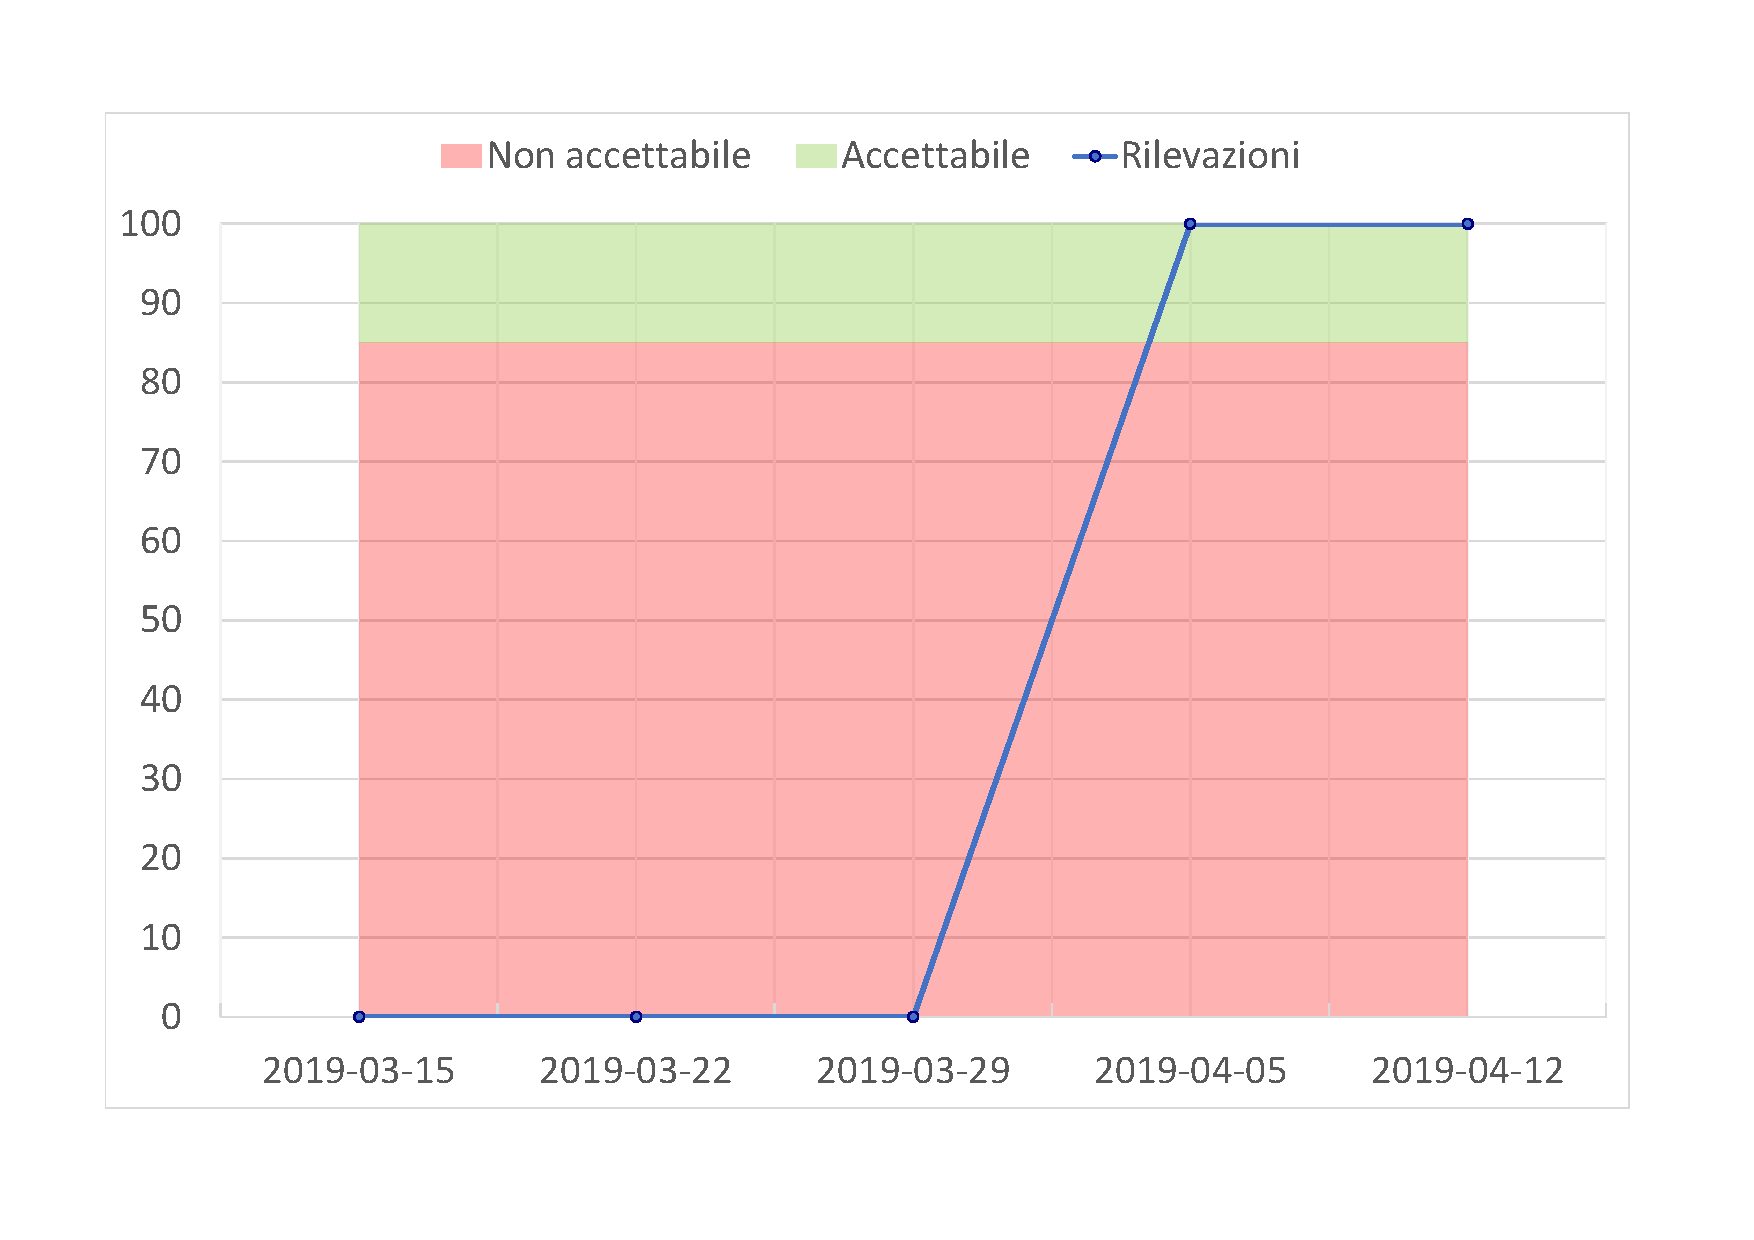
\includegraphics[scale=0.6]{images/resoconto/MPS1Chart.pdf}
	\caption{Serie storica percentuale di superamento test}	
\end{figure}

\paragraph{Numero di parametri per metodo - MPS2}
\subparagraph{Codifica al 2019-04-05}
In questo periodo dell'attività di codifica, la media di parametri per metodo equivale a 1. Infatti sono stati implementati 75 metodi con un totale di 95 parametri.

\subparagraph{Codifica al 2019-04-12}
In questo periodo dell'attività di codifica, la media di parametri per metodo è inferiore a 1. Infatti sono stati implementati 74 metodi con un totale di 44 parametri per un totale di 149 metodi e 139 parametri.

\subparagraph{Codifica al 2019-04-19}
In questo periodo dell'attività di codifica, la media di parametri per metodo è 0.93. Infatti sono stati implementati 9 metodi con un totale di 10 parametri per un totale di 158 metodi e 148 parametri.

\subparagraph{Codifica al 2019-04-26}
In questo periodo dell'attività di codifica, la media di parametri per metodo è 0.94. Infatti sono stati implementati 9 metodi con un totale di 9 parametri per un totale di 167 metodi e 157 parametri.

\subparagraph{Codifica al 2019-05-03}
In questo periodo dell'attività di codifica, la media di parametri per metodo è 0.91. Infatti sono stati implementati 5 metodi con  0 parametri per un totale di 172 metodi e 157 parametri. 
A seguito di questa attività di codifica, il prodotto si ritiene concluso all'implementazione.

\subparagraph{Codifica al 2019-05-10}
In questo periodo non si è verificata l'attività di codifica in quanto il prodotto è stato ritenuto concluso precedentemente.
\\
\begin{figure}[H]
	\centering
	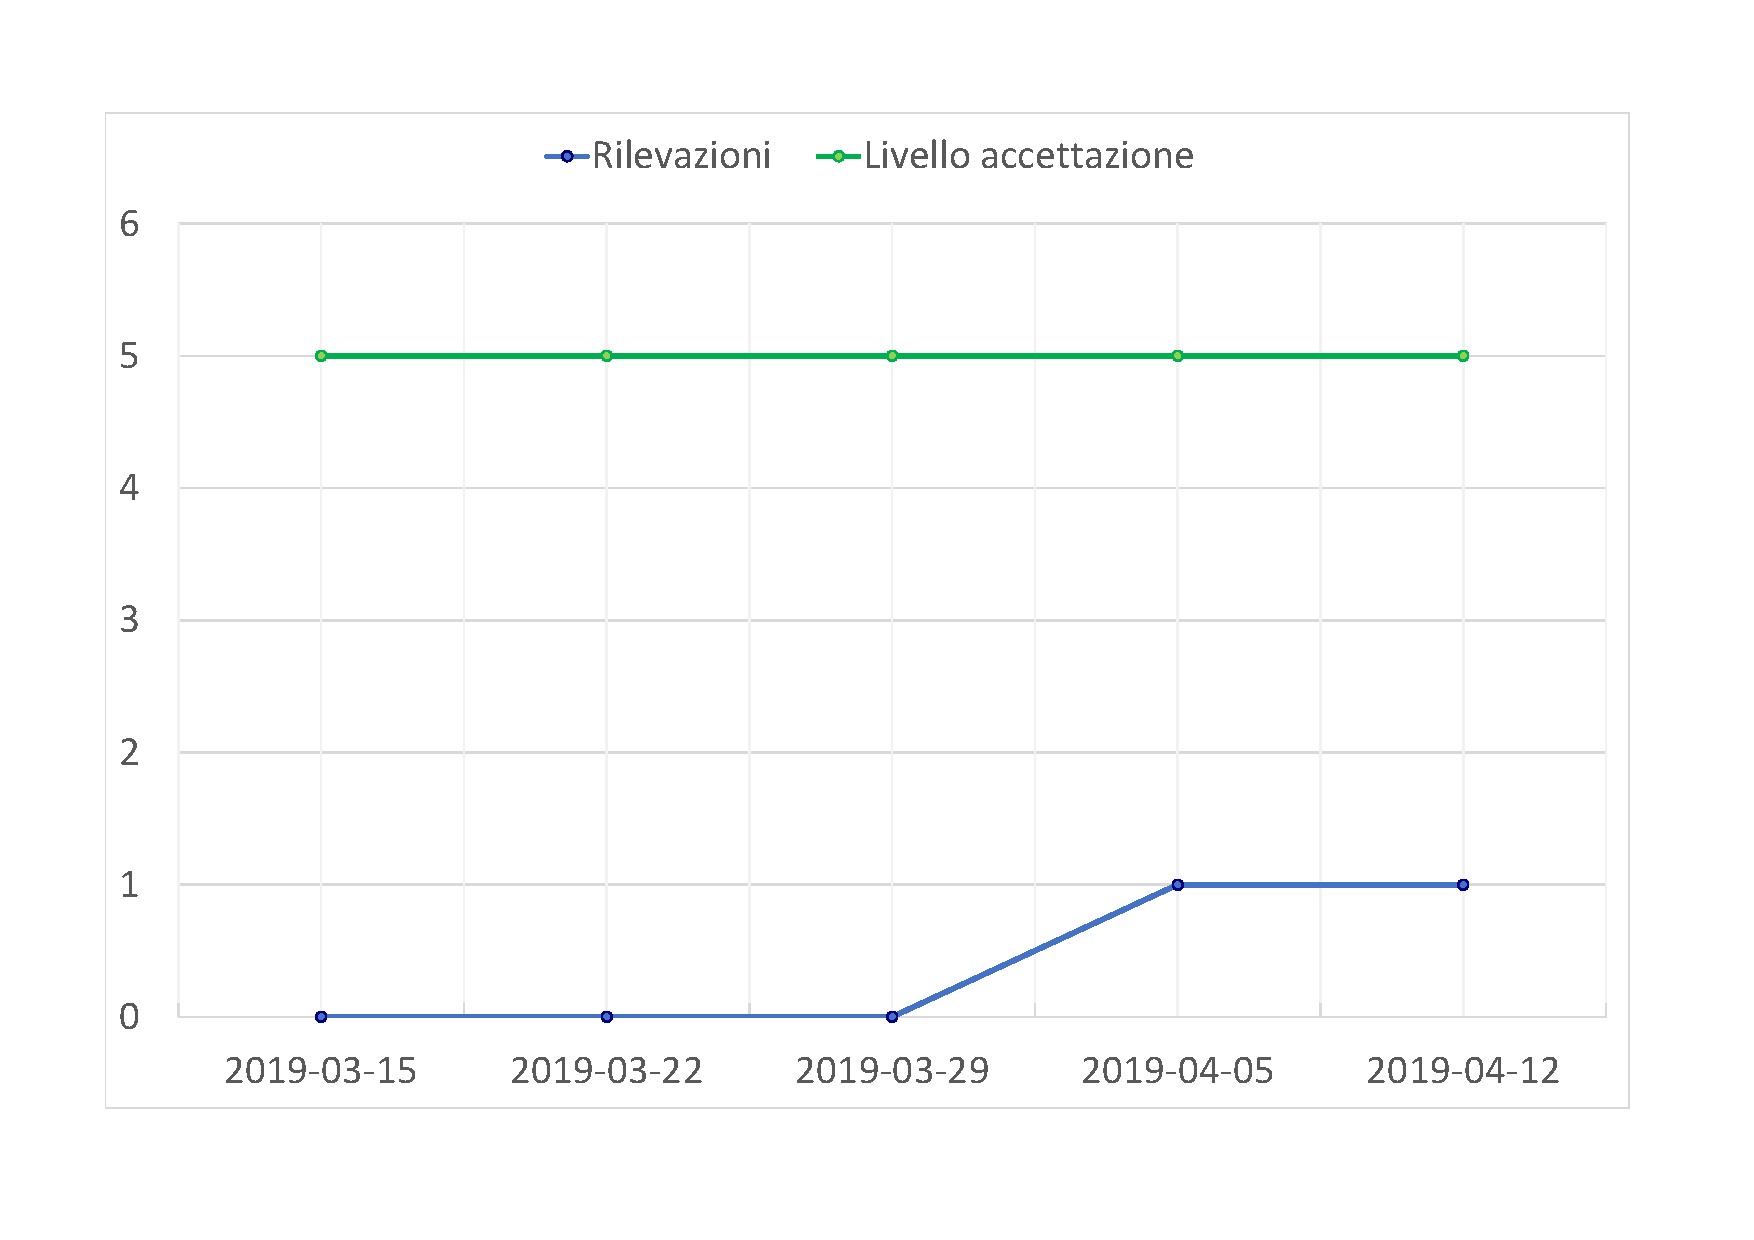
\includegraphics[scale=0.6]{images/resoconto/MPS2Chart.pdf}
	\caption{Serie storica numero di parametri per metodo}	
\end{figure}

\paragraph{Numero di attributi per classe - MPS3}
\subparagraph{Codifica al 2019-04-05}
In questo periodo dell'attività di codifica, la media di attributi per classe equivale a 2. Infatti sono stati implementate 23 classi con un totale di 37 attributi.

\subparagraph{Codifica al 2019-04-12}
In questo periodo dell'attività di codifica, la media di attributi per classe equivale a 1.30. Infatti sono stati implementate 10 classi con un totale di 7 attributi per un totale di 33 classi e 43 attributi.

\subparagraph{Codifica al 2019-04-19}
In questo periodo dell'attività di codifica, la media di attributi per classe equivale a 1.30. Infatti non è stata implementata completamente una classe e il totale di classi implementate rimane a 33 con 43 attributi.

\subparagraph{Codifica al 2019-04-26}
In questo periodo dell'attività di codifica, la media di attributi per classe è 1.35. Infatti è stata implementata 1 classe con 3 attributi per un totale di 34 classi e 46 attributi.

\subparagraph{Codifica al 2019-05-03}
In questo periodo dell'attività di codifica, la media di attributi per classe è 1.35. Infatti è stata implementata 1 classe con 3 attributi per un totale di 35 classi e 46 attributi.
A seguito di questa attività di codifica, il prodotto si ritiene concluso all'implementazione.

\subparagraph{Codifica al 2019-05-10}
In questo periodo non si è verificata l'attività di codifica in quanto il prodotto è stato ritenuto concluso precedentemente.

\begin{figure}[H]
	\centering
	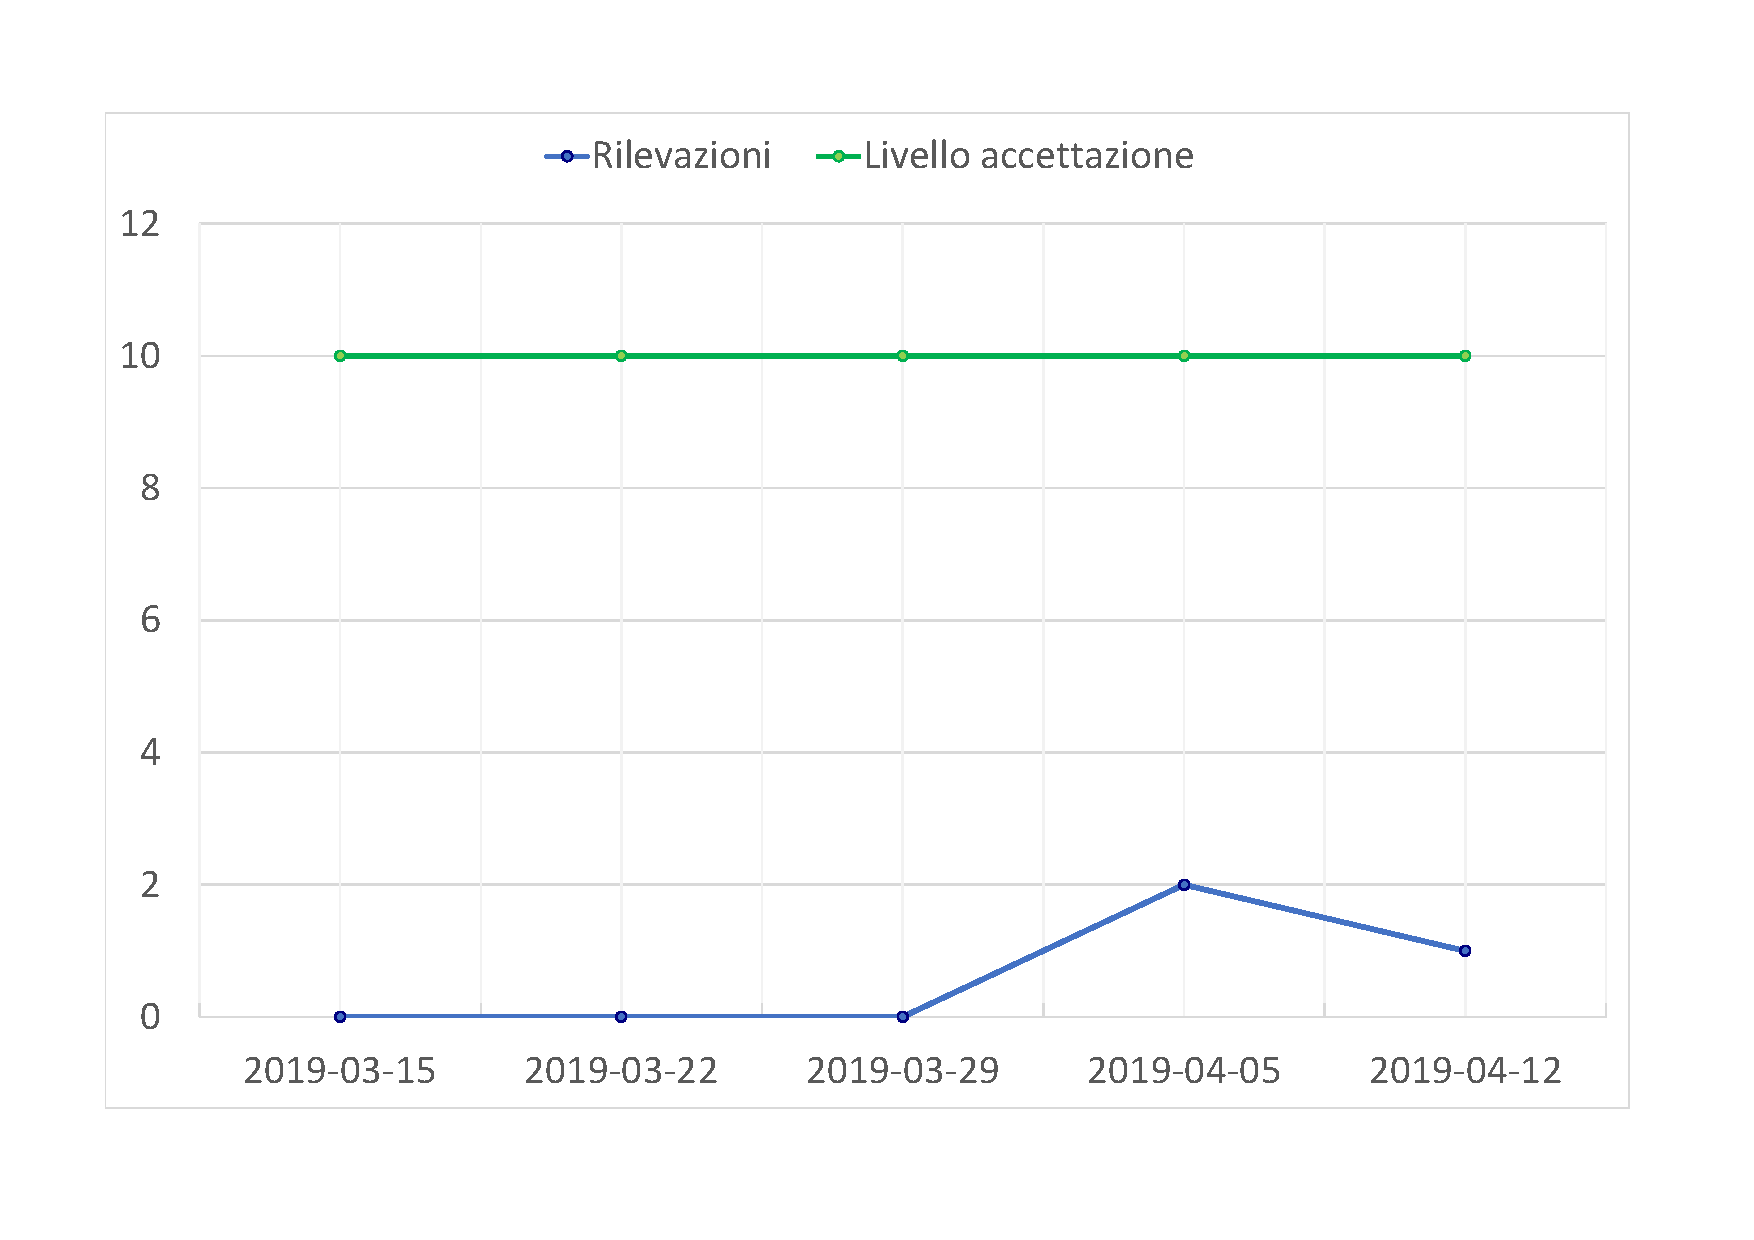
\includegraphics[scale=0.6]{images/resoconto/MPS3Chart.pdf}
	\caption{Serie storica numero di attributi per classe}	
\end{figure}

\paragraph{Numero di metodi per classe - MPS4}
\subparagraph{Codifica al 2019-04-05}
In questo periodo dell'attività di codifica, la media di metodi per classe equivale a 3. Infatti sono stati implementate 23 classi con un totale di 75 metodi.

\subparagraph{Codifica al 2019-04-12}
In questo periodo dell'attività di codifica, la media di metodi per classe equivale a 4.5. Infatti sono state implementate 10 classi con un totale di 74 metodi per un totale di 33 classi e 149 metodi.

\subparagraph{Codifica al 2019-04-19}
In questo periodo dell'attività di codifica, la media di metodi per classe equivale a 4.5. Infatti non è stata implementata completamente una classe e il totale di classi implementate rimane a 33 con 149 metodi.

\subparagraph{Codifica al 2019-04-26}
In questo periodo dell'attività di codifica, la media di metodi per classe equivale a 5. Infatti è stata implementata 1 classe con un totale di 18 metodi per un totale di 34 classi e 167 metodi.

\subparagraph{Codifica al 2019-05-03}
In questo periodo dell'attività di codifica, la media di metodi per classe equivale a 5. Infatti è stata implementata 1 classe con un totale di 5 metodi per un totale di 35 classi e 172 metodi.

\subparagraph{Codifica al 2019-05-10}
In questo periodo non si è verificata l'attività di codifica in quanto il prodotto è stato ritenuto concluso precedentemente.

\begin{figure}[H]
	\centering
	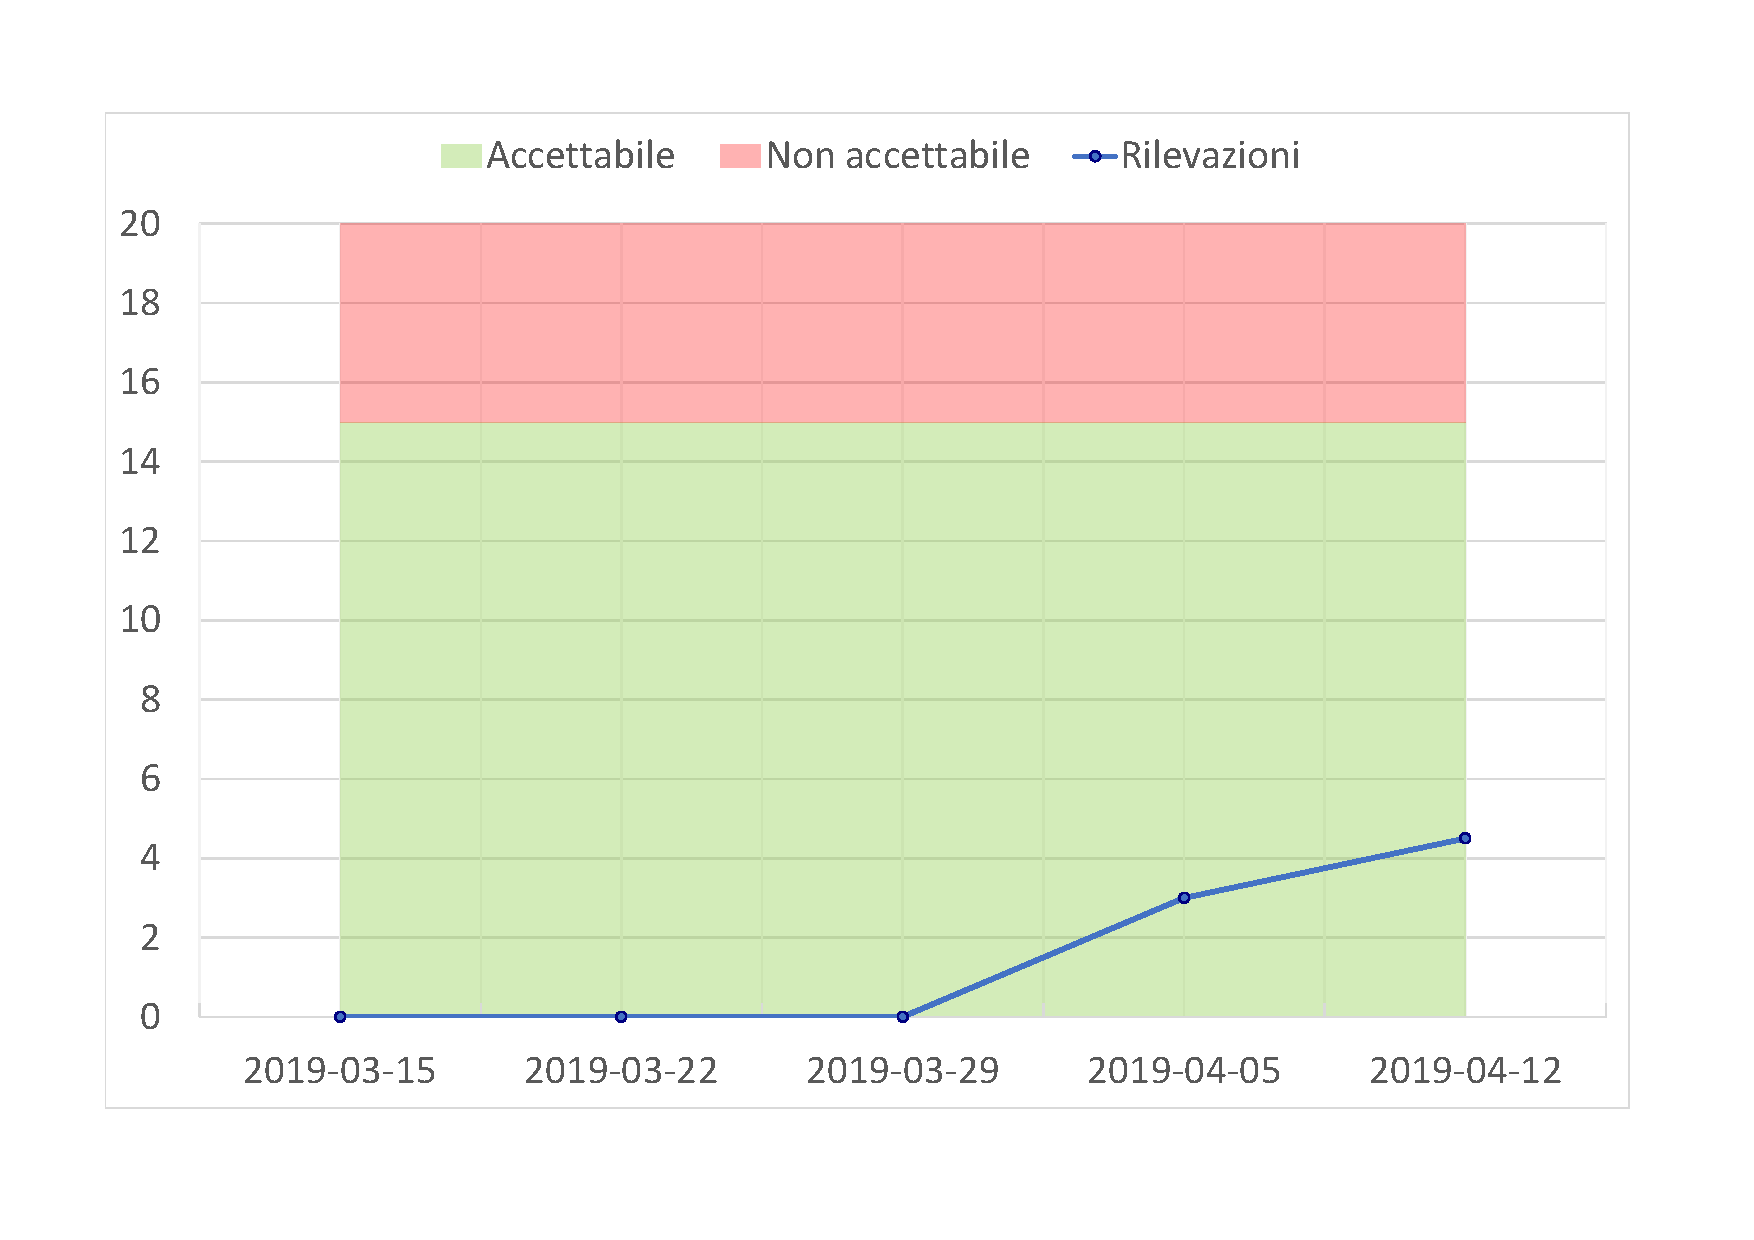
\includegraphics[scale=0.6]{images/resoconto/MPS4Chart.pdf}
	\caption{Serie storica rilevazioni numero di metodi per classe}	
\end{figure}

\paragraph{Complessità ciclomatica media - MPS5}
\subparagraph{Codifica al 2019-04-05}
In questo periodo dell'attività di codifica, la complessità ciclomatica media di 74 metodi sviluppati è di circa 1.61. 

\subparagraph{Codifica al 2019-04-12}
In questo periodo dell'attività di codifica, son stati sviluppati 75 metodi, con un totale di 149 e un indice di complessità ciclomatica media di circa 1.20.

\subparagraph{Codifica al 2019-04-19}
In questo periodo dell'attività di codifica, la complessità ciclomatica media di 149 metodi sviluppati è di circa 1.22. 

\subparagraph{Codifica al 2019-04-26}
In questo periodo dell'attività di codifica, la complessità ciclomatica media di 167 metodi sviluppati è di circa 1.35. 

\subparagraph{Codifica al 2019-05-03}
In questo periodo dell'attività di codifica, la complessità ciclomatica media di 172 metodi sviluppati è di circa 1.28. 

\subparagraph{Codifica al 2019-05-10}
In questo periodo non si è verificata l'attività di codifica in quanto il prodotto è stato ritenuto concluso precedentemente.

\begin{figure}[H]
	\centering
	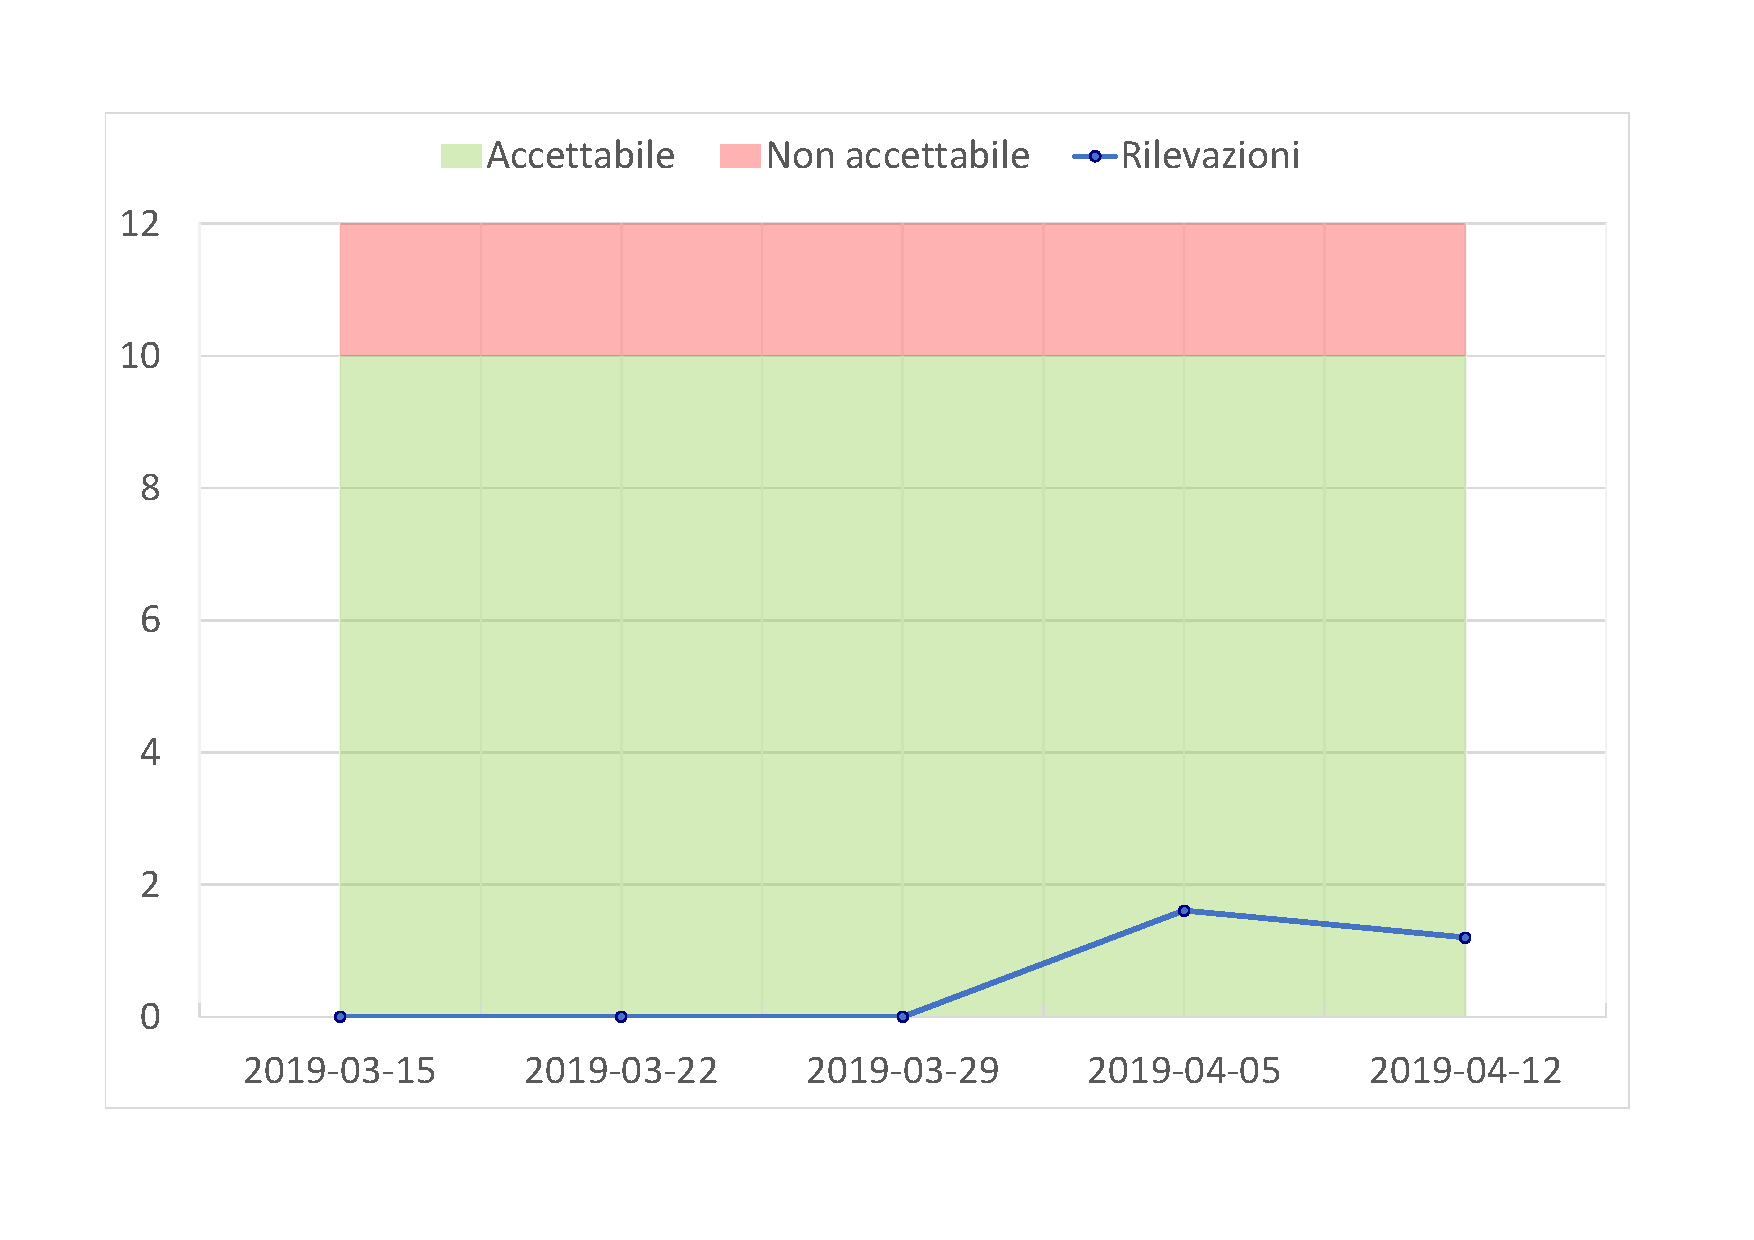
\includegraphics[scale=0.6]{images/resoconto/MPS5Chart.pdf}
	\caption{Serie storica rilevazioni numero di metodi per classe}	
\end{figure}


\paragraph{Implementazione dei requisiti obbligatori - MPS6}
\subparagraph{Codifica al 2019-04-05}
In questo periodo dell'attività di codifica, sono stati soddisfatti 26 requisiti obbligatori, ovvero il 56,52\% dei requisiti obbligatori totali.
Nonostante non raggiunga il livello di accettazione della
metrica, questo risultato è ritenuto sufficiente a questo punto del progetto poiché sono previsti altri incrementi alla codifica che porteranno al soddisfacimento di altri requisiti.

\subparagraph{Codifica al 2019-04-12}
In questo periodo dell'attività di codifica, sono stati soddisfatti 12 requisiti obbligatori, per un totale di 38, ovvero l'82,60\% dei requisiti obbligatori totali.
Nonostante non raggiunga il livello di accettazione della
metrica, questo risultato è ritenuto sufficiente a questo punto del progetto poiché sono previsti altri incrementi alla codifica che porteranno al soddisfacimento di altri requisiti.

\subparagraph{Codifica al 2019-04-19}
In questo periodo dell'attività di codifica, sono stati soddisfatti 12 requisiti obbligatori, per un totale di 40, ovvero l'86.95\% dei requisiti obbligatori totali.
Nonostante non raggiunga il livello di accettazione della
metrica, questo risultato è ritenuto sufficiente a questo punto del progetto poiché sono previsti altri incrementi alla codifica che porteranno al soddisfacimento di altri requisiti.

\subparagraph{Codifica al 2019-04-26}
In questo periodo dell'attività di codifica, sono stati soddisfatti 12 requisiti obbligatori, per un totale di 43, ovvero il 93.48\% dei requisiti obbligatori totali.
Nonostante non raggiunga il livello di accettazione della
metrica, questo risultato è ritenuto sufficiente a questo punto del progetto poiché sono previsti altri incrementi alla codifica che porteranno al soddisfacimento di altri requisiti.

\subparagraph{Codifica al 2019-05-03}
In questo periodo dell'attività di codifica, sono stati soddisfatti 12 requisiti obbligatori, per un totale di 46, ovvero il 100\% dei requisiti obbligatori totali.
A seguito di questo periodo di codifica la soglia di accettabilità della metrica è stata raggiunta.

\subparagraph{Codifica al 2019-05-10}
In questo periodo non si è verificata l'attività di codifica in quanto il prodotto è stato ritenuto concluso precedentemente.

\begin{figure}[H]
	\centering
	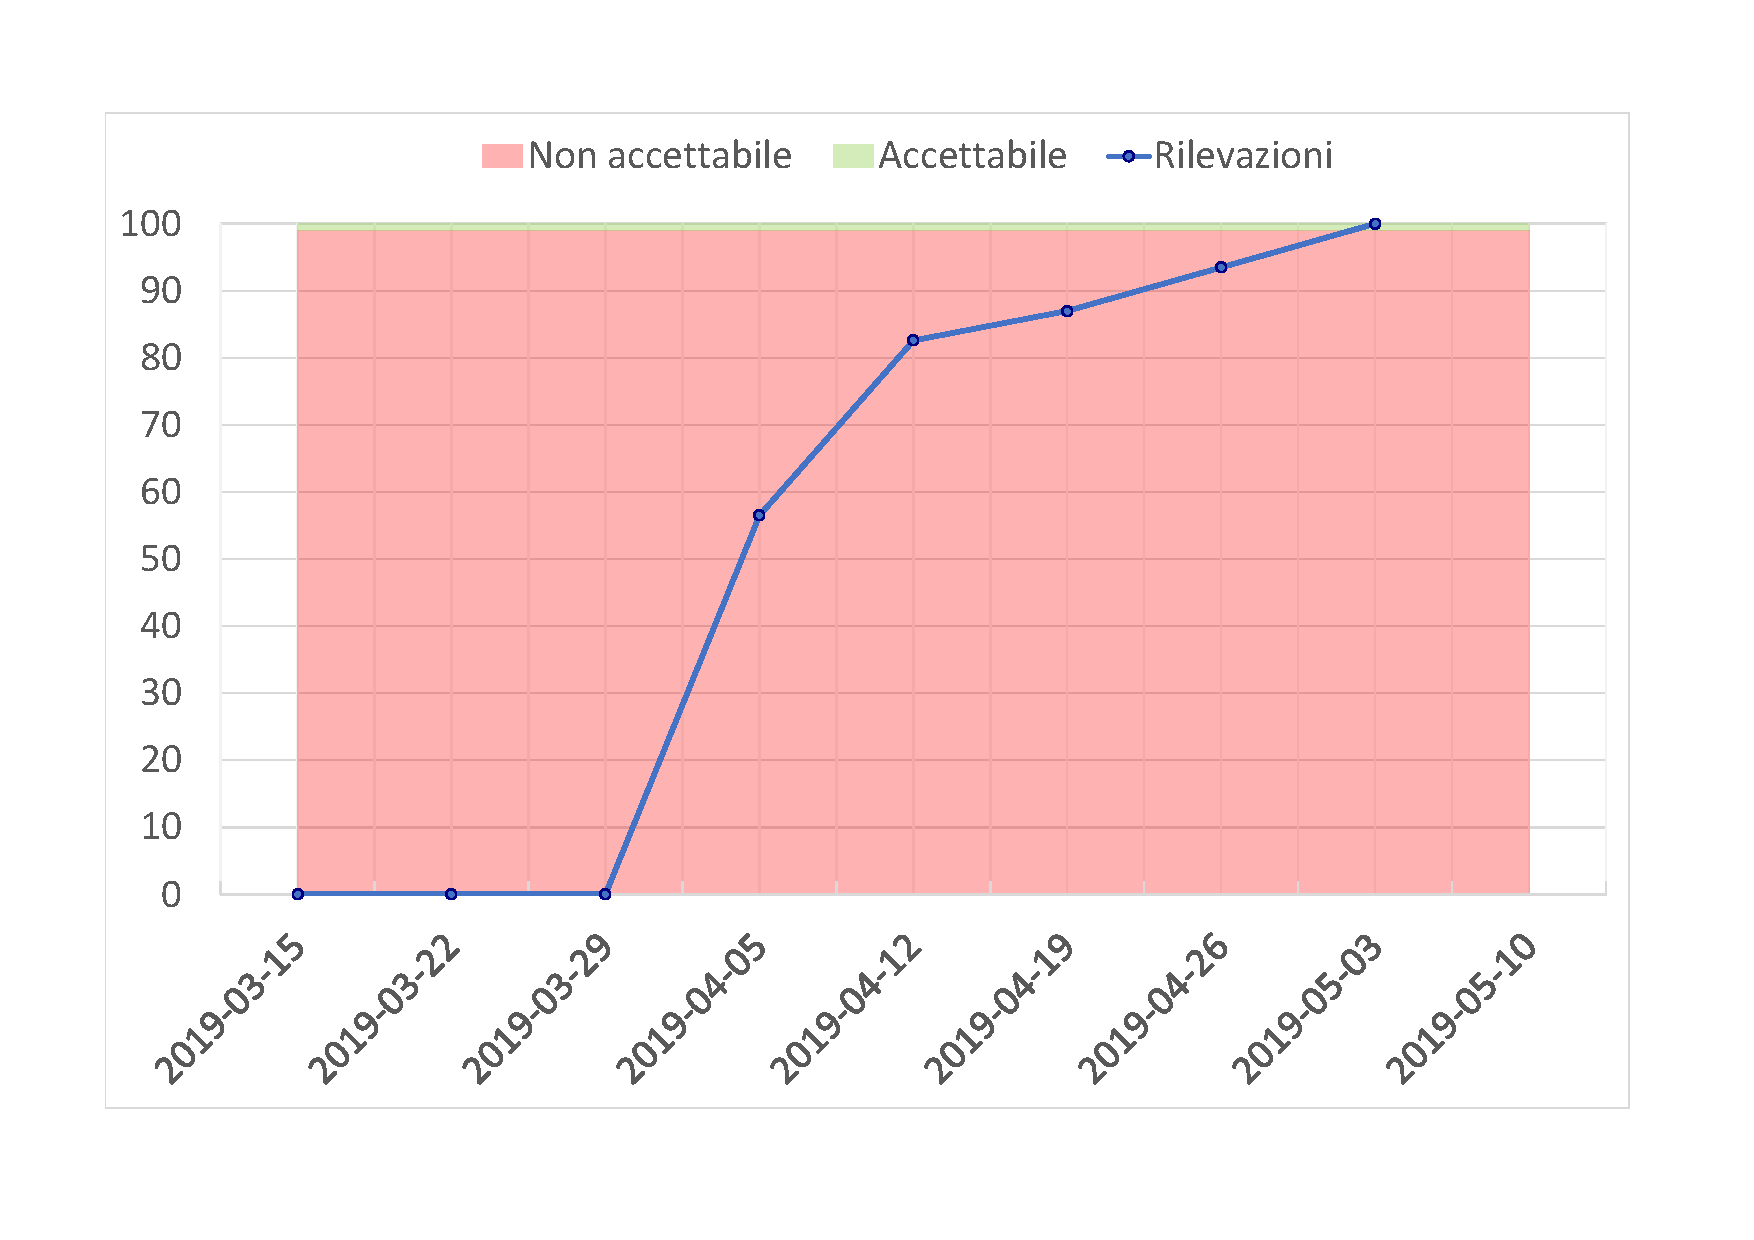
\includegraphics[scale=0.6]{images/resoconto/MPS6Chart.pdf}
	\caption{Serie storica percentuale di requisiti obbligatori soddisfatti}	
\end{figure}

\paragraph{Implementazione dei requisiti desiderabili - MPS7}
\subparagraph{Codifica al 2019-04-05}
In questo periodo dell'attività di codifica, sono stati soddisfatti 6 requisiti desiderabili, ovvero il 13,63\% dei requisiti desiderabili totali.
Nonostante non raggiunga il livello di accettazione della
metrica, questo risultato è ritenuto sufficiente a questo punto del progetto poiché sono previsti altri incrementi alla codifica che porteranno al soddisfacimento di altri requisiti.

\subparagraph{Codifica al 2019-04-12}
In questo periodo dell'attività di codifica, sono stati soddisfatti 4 requisiti desiderabili, per un totale di 10, ovvero il 22,72\% dei requisiti desiderabili totali.
Nonostante non raggiunga il livello di accettazione della
metrica, questo risultato è ritenuto sufficiente a questo punto del progetto poiché sono previsti altri incrementi alla codifica che porteranno al soddisfacimento di altri requisiti.

\subparagraph{Codifica al 2019-04-19}
In questo periodo dell'attività di codifica, sono stati soddisfatti 5 requisiti desiderabili, per un totale di 15, ovvero il 30,61\% dei requisiti desiderabili totali.
A seguito di questo periodo di codifica la soglia di accettabilità della metrica è stata raggiunta.
Il gruppo si impegnerà ad incrementare ulteriormente la copertura di altri requisiti desiderabili.

\subparagraph{Codifica al 2019-04-26}
In questo periodo dell'attività di codifica, sono stati soddisfatti 4 requisiti desiderabili, per un totale di 19, ovvero il 38,77\% dei requisiti desiderabili totali.

\subparagraph{Codifica al 2019-05-03}
In questo periodo dell'attività di codifica, sono stati soddisfatti 6 requisiti desiderabili, per un totale di 25, ovvero il 51,02\% dei requisiti desiderabili totali.

\subparagraph{Codifica al 2019-05-10}
In questo periodo non si è verificata l'attività di codifica in quanto il prodotto è stato ritenuto concluso precedentemente.

\begin{figure}[H]
	\centering
	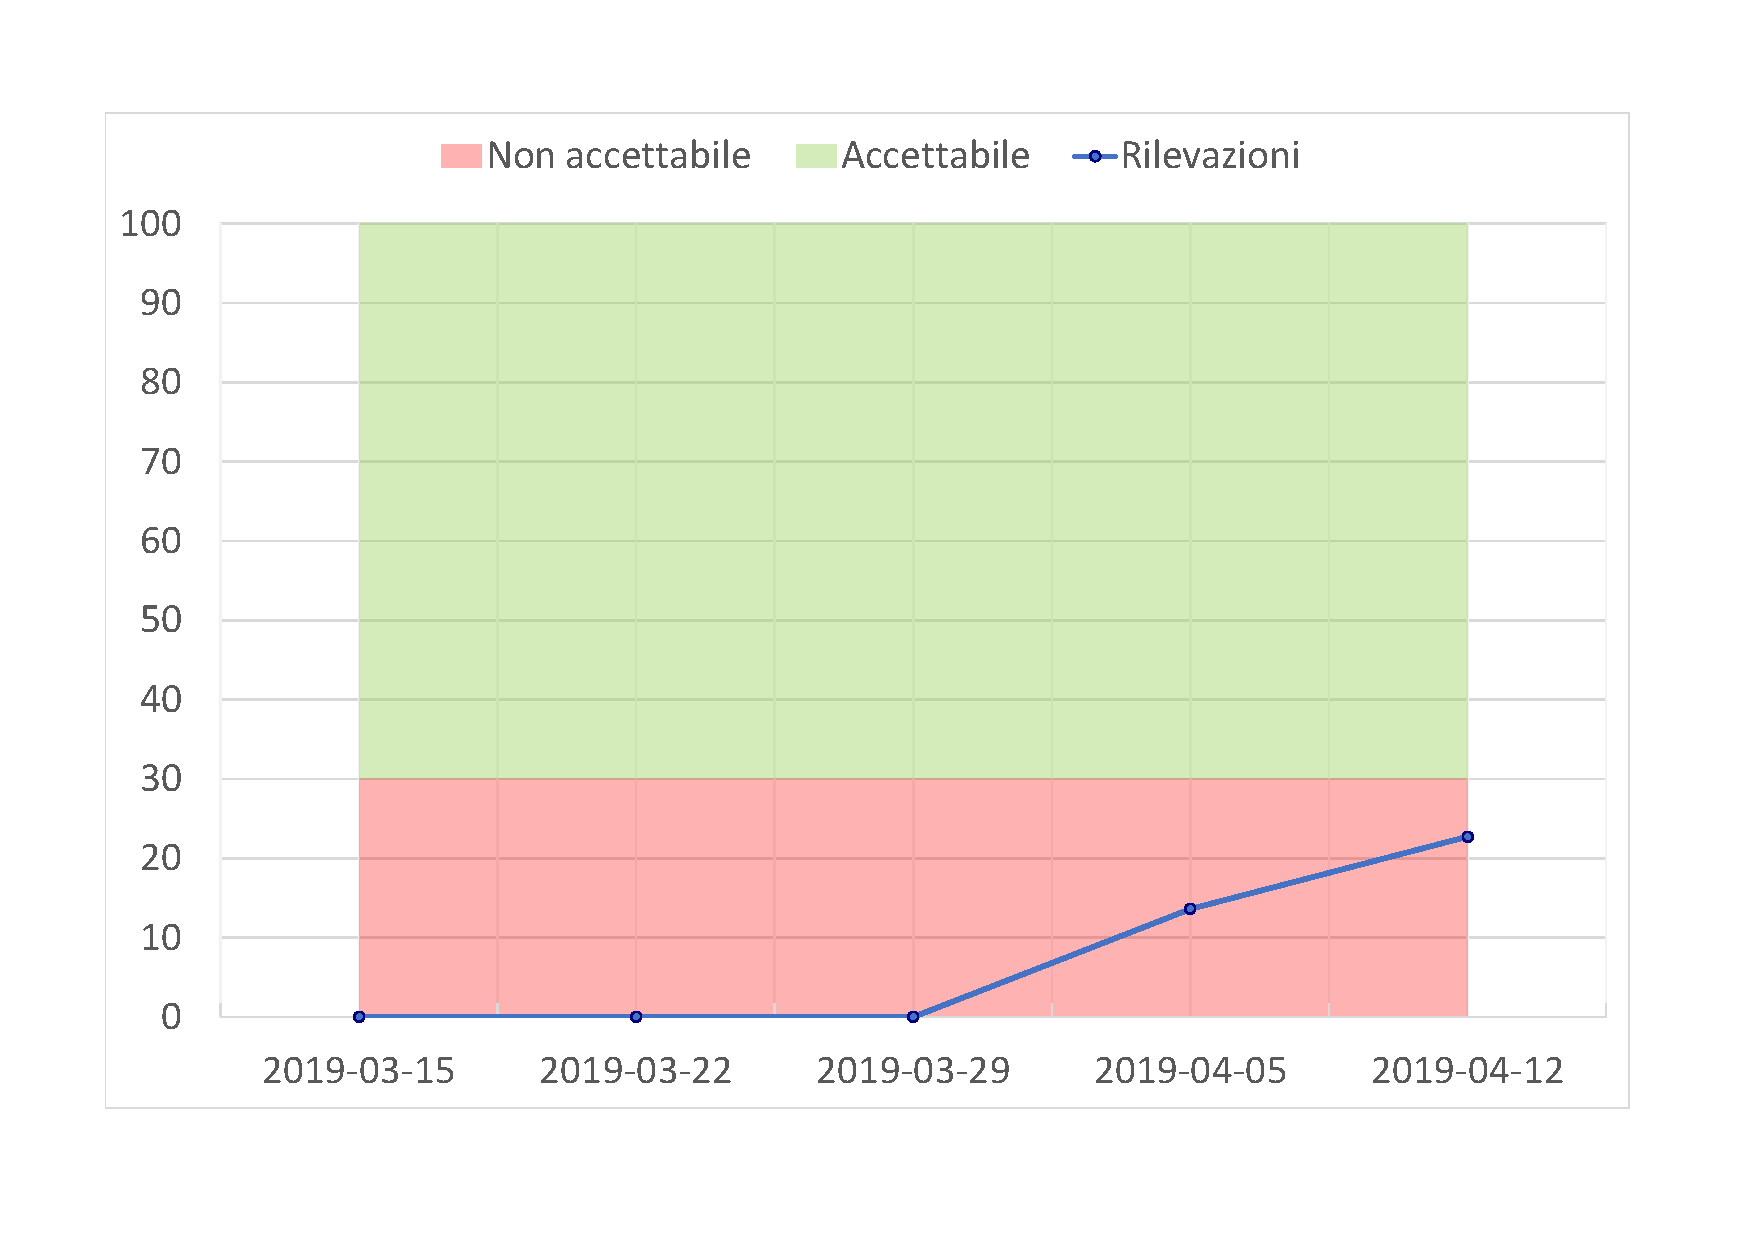
\includegraphics[scale=0.6]{images/resoconto/MPS7Chart.pdf}
	\caption{Serie storica percentuale di requisiti desiderabili soddisfatti}	
\end{figure}

\paragraph{Copertura dei test sul codice - MPS8}
\subparagraph{Codifica al 2019-04-05}
In questo periodo dell'attività di codifica, sono stati implementati 21 test, coprendo circa il 92.47\% degli statements delle classi testate.

\subparagraph{Codifica al 2019-04-12}
In questo periodo dell'attività di codifica, sono stati implementati 21 test, con un totale di 42 test coprendo circa il 89.98\% degli statements delle classi testate.

\subparagraph{Codifica al 2019-04-19}

\subparagraph{Codifica al 2019-04-26}

\subparagraph{Codifica al 2019-05-03}

\subparagraph{Codifica al 2019-05-10}

\begin{figure}[H]
	\centering
	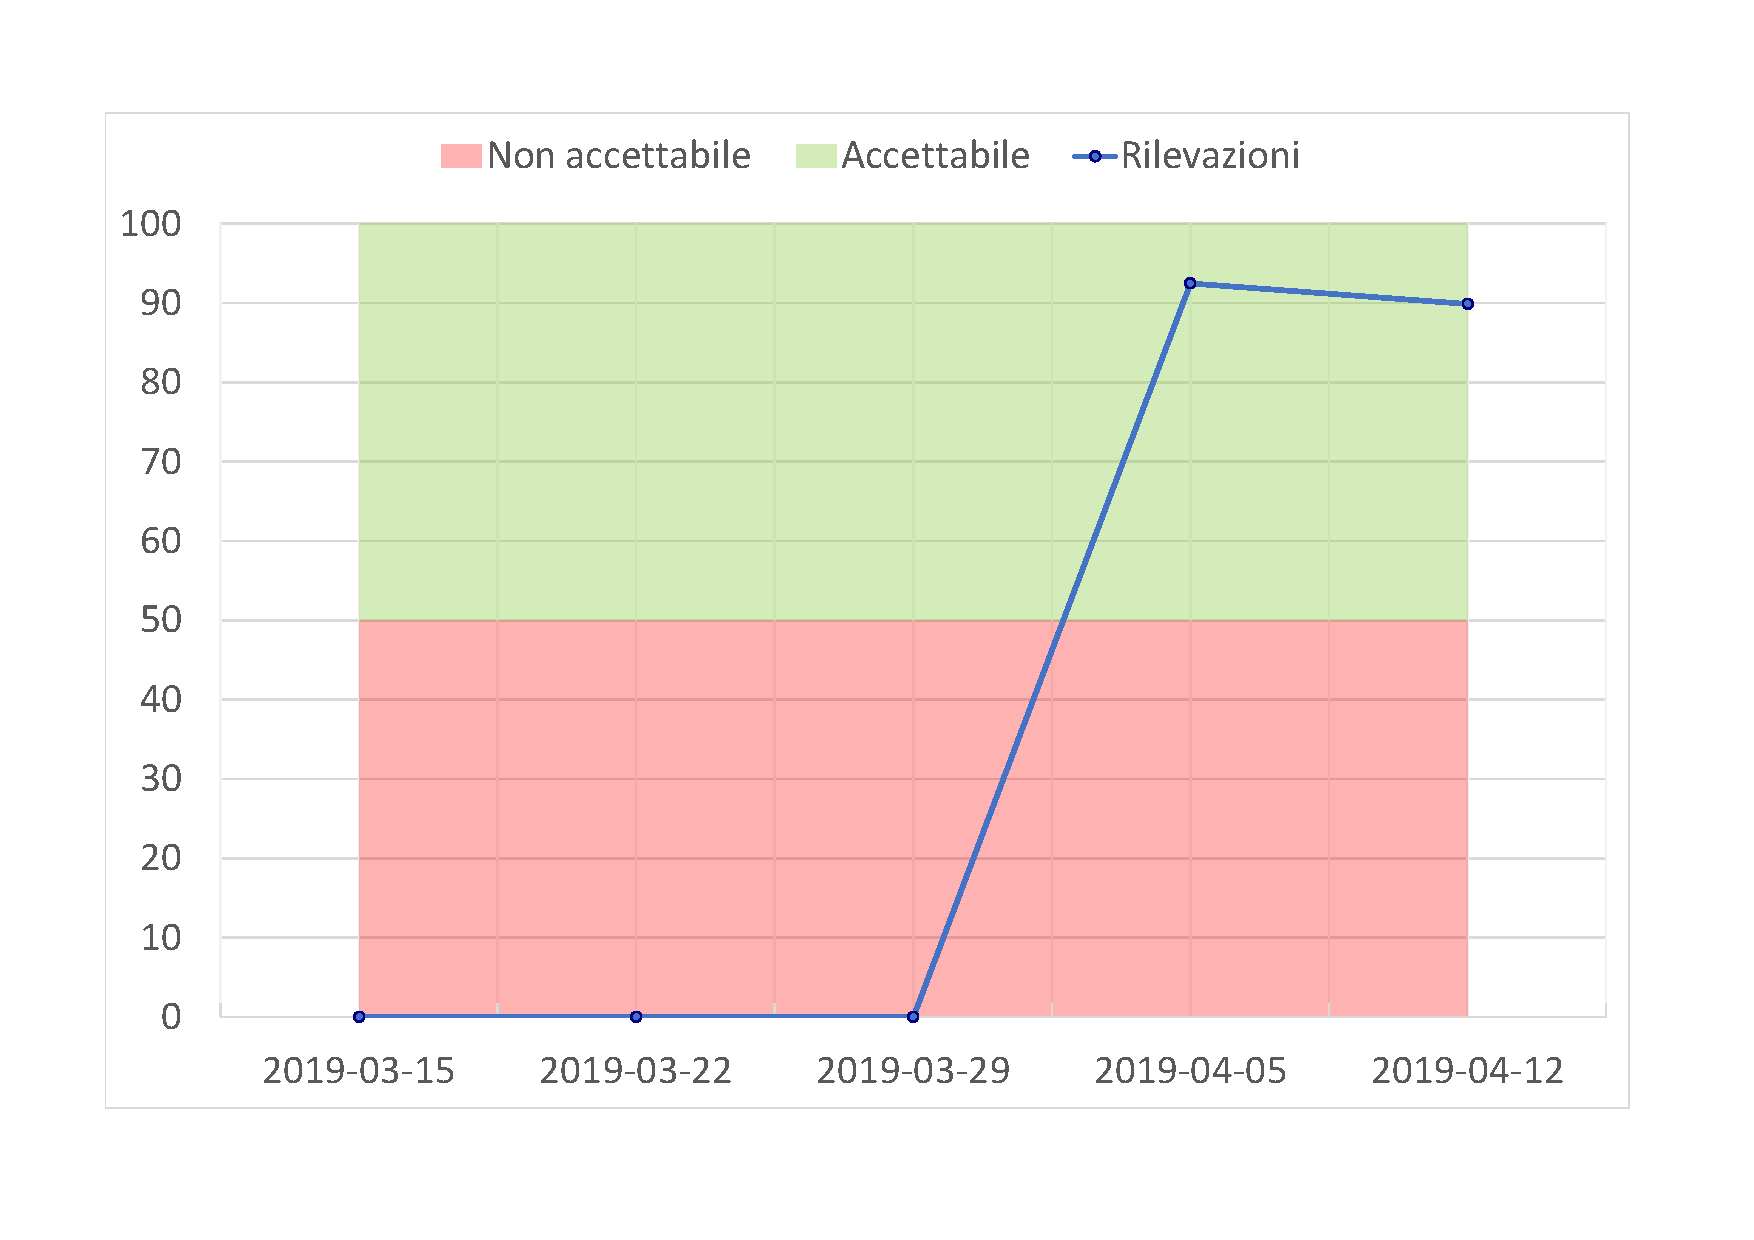
\includegraphics[scale=0.6]{images/resoconto/MPS8Chart.pdf}
	\caption{Serie storica rilevazioni copertura dei test sul codice}	
\end{figure}


\paragraph{Implementazione dei requisiti opzionali - MPS9}
\subparagraph{Codifica al 2019-04-05}
In questo periodo dell'attività di codifica, sono stati soddisfatti 0 requisiti opzionali. Il valore della metrica rimane a 0.

\subparagraph{Codifica al 2019-04-12}
In questo periodo dell'attività di codifica, sono stati soddisfatti 2 requisiti opzionali, ovvero il 6,25\% dei requisiti opzionali totali.
Nonostante non raggiunga il livello di accettazione della
metrica, questo risultato è ritenuto sufficiente a questo punto del progetto poiché sono previsti altri incrementi alla codifica che porteranno al soddisfacimento di altri requisiti.

\subparagraph{Codifica al 2019-04-19}
In questo periodo dell'attività di codifica, sono stati soddisfatti 2 requisiti opzionali, con un totale di 4 requisiti totali implementati, ovvero il 12.50\% dei requisiti opzionali totali.
A seguito di questo periodo di codifica la soglia di accettabilità della metrica è stata raggiunta.
Il gruppo si impegnerà ad incrementare ulteriormente la copertura di altri requisiti opzionali.

\subparagraph{Codifica al 2019-04-26}
In questo periodo dell'attività di codifica, sono stato soddisfatto 1 requisito opzionale, con un totale di 5 requisiti totali implementati, ovvero il 15.63\% dei requisiti opzionali totali.

\subparagraph{Codifica al 2019-05-03}
In questo periodo dell'attività di codifica, sono stato soddisfatto 1 requisito opzionale, con un totale di 6 requisiti totali implementati, ovvero il 18.75\% dei requisiti opzionali totali.

\subparagraph{Codifica al 2019-05-10}
In questo periodo non si è verificata l'attività di codifica in quanto il prodotto è stato ritenuto concluso precedentemente.

\begin{figure}[H]
	\centering
	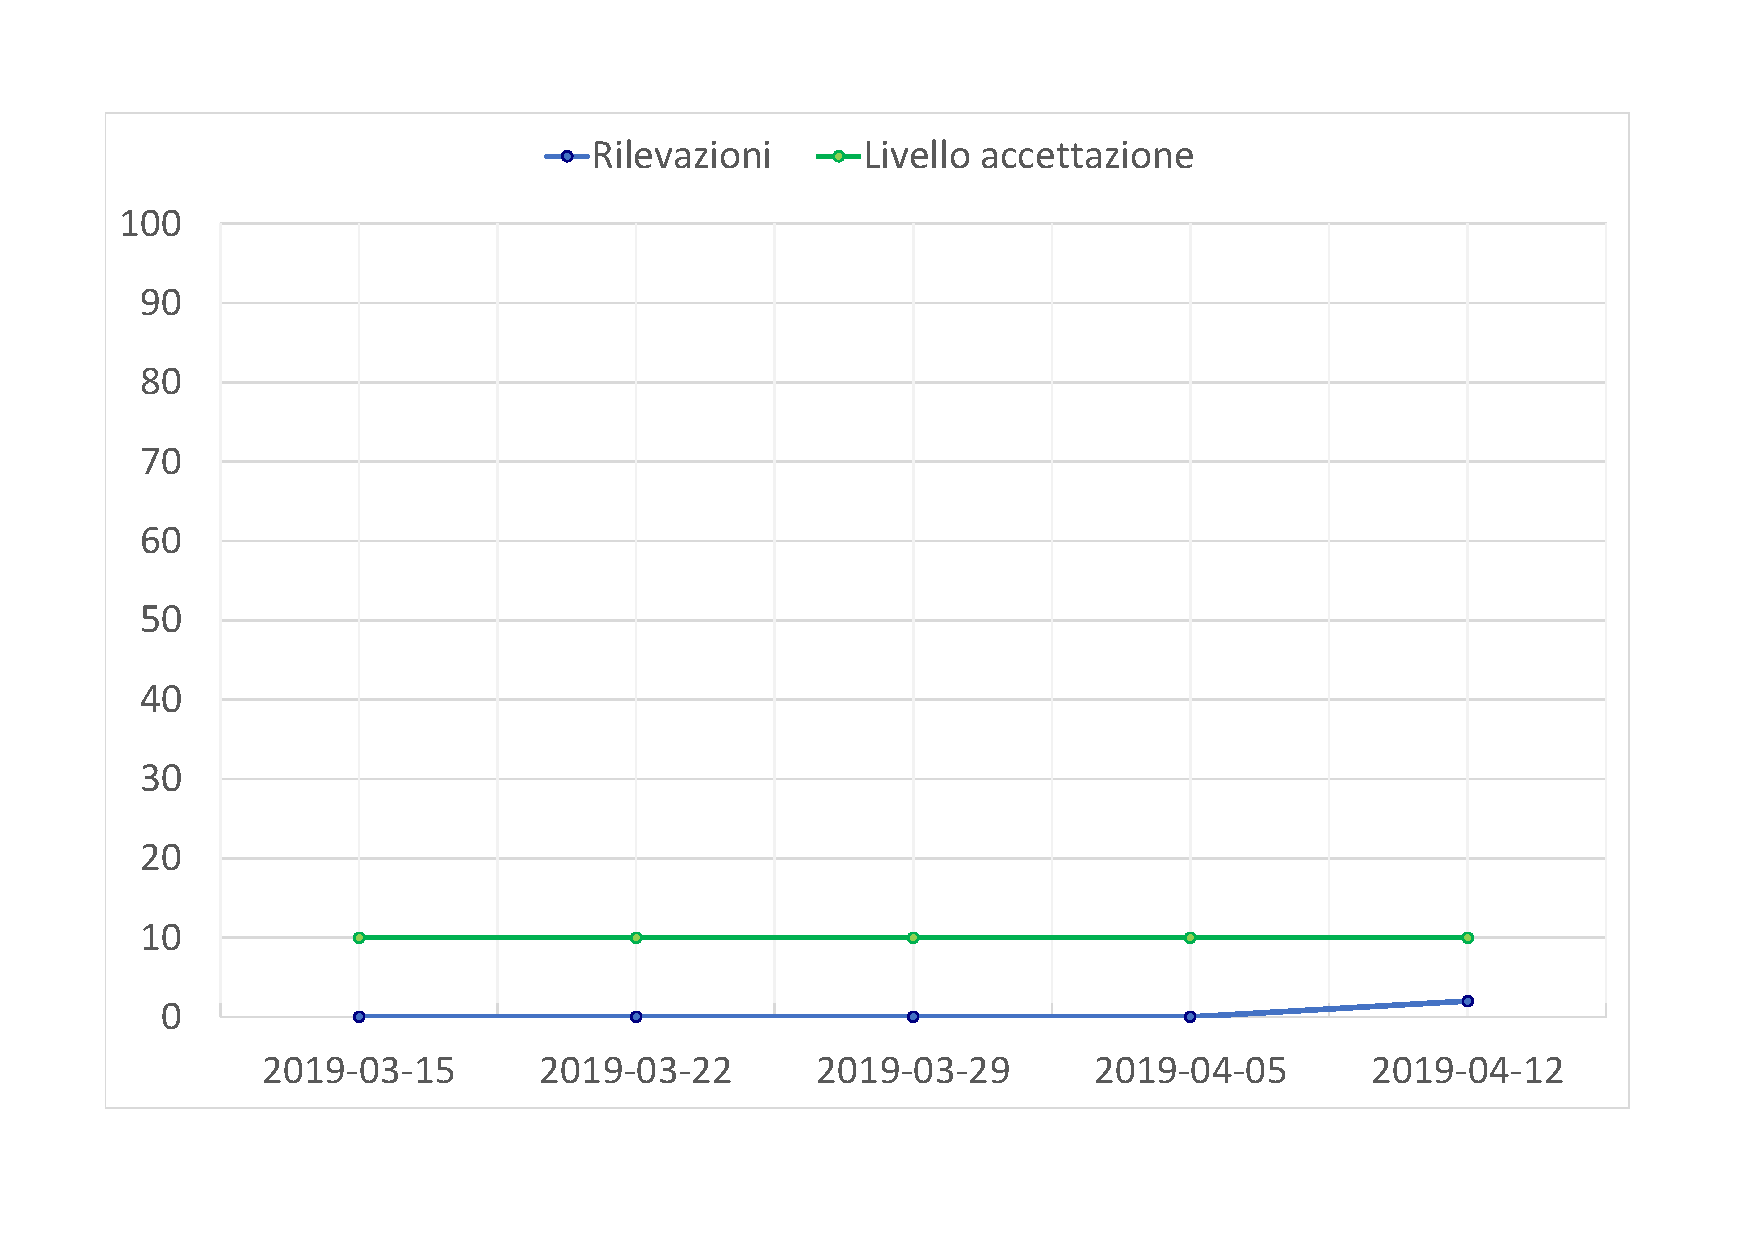
\includegraphics[scale=0.6]{images/resoconto/MPS9Chart.pdf}
	\caption{Serie storica percentuale di requisiti opzionali soddisfatti}	
\end{figure}

\paragraph{Numero di linee di codice di una procedura - MPS10}
\subparagraph{Codifica al 2019-04-05}
In questo periodo dell'attività di codifica, la media di linee di codice per procedura equivale a 20. Infatti sono stati implementati 75 metodi con un totale di circa 1500 linee di codice.

\subparagraph{Codifica al 2019-04-12}
In questo periodo dell'attività di codifica, la media di linee di codice per procedura equivale a 16.77. Infatti sono stati implementati 74 metodi con un totale di circa 1000 linee di codice, per un totale di 149 metodi e 2500 linee di codice.

\subparagraph{Codifica al 2019-04-19}
In questo periodo dell'attività di codifica, la media di linee di codice per procedura equivale a 16.50. Infatti sono stati implementati 9 metodi con un totale di circa 130 linee di codice, per un totale di 158 metodi e 2630 linee di codice.

\subparagraph{Codifica al 2019-04-26}
In questo periodo dell'attività di codifica, la media di linee di codice per procedura equivale a 16.35. Infatti sono stati implementati 9 metodi con un totale di circa 100 linee di codice, per un totale di 167 metodi e 2730 linee di codice.

\subparagraph{Codifica al 2019-05-03}
In questo periodo dell'attività di codifica, la media di linee di codice per procedura equivale a 16.31. Infatti sono stati implementati 5 metodi con un totale di circa 75 linee di codice, per un totale di 172 metodi e 2805 linee di codice.

\subparagraph{Codifica al 2019-05-10}
In questo periodo non si è verificata l'attività di codifica in quanto il prodotto è stato ritenuto concluso precedentemente.

\begin{figure}[H]
	\centering
	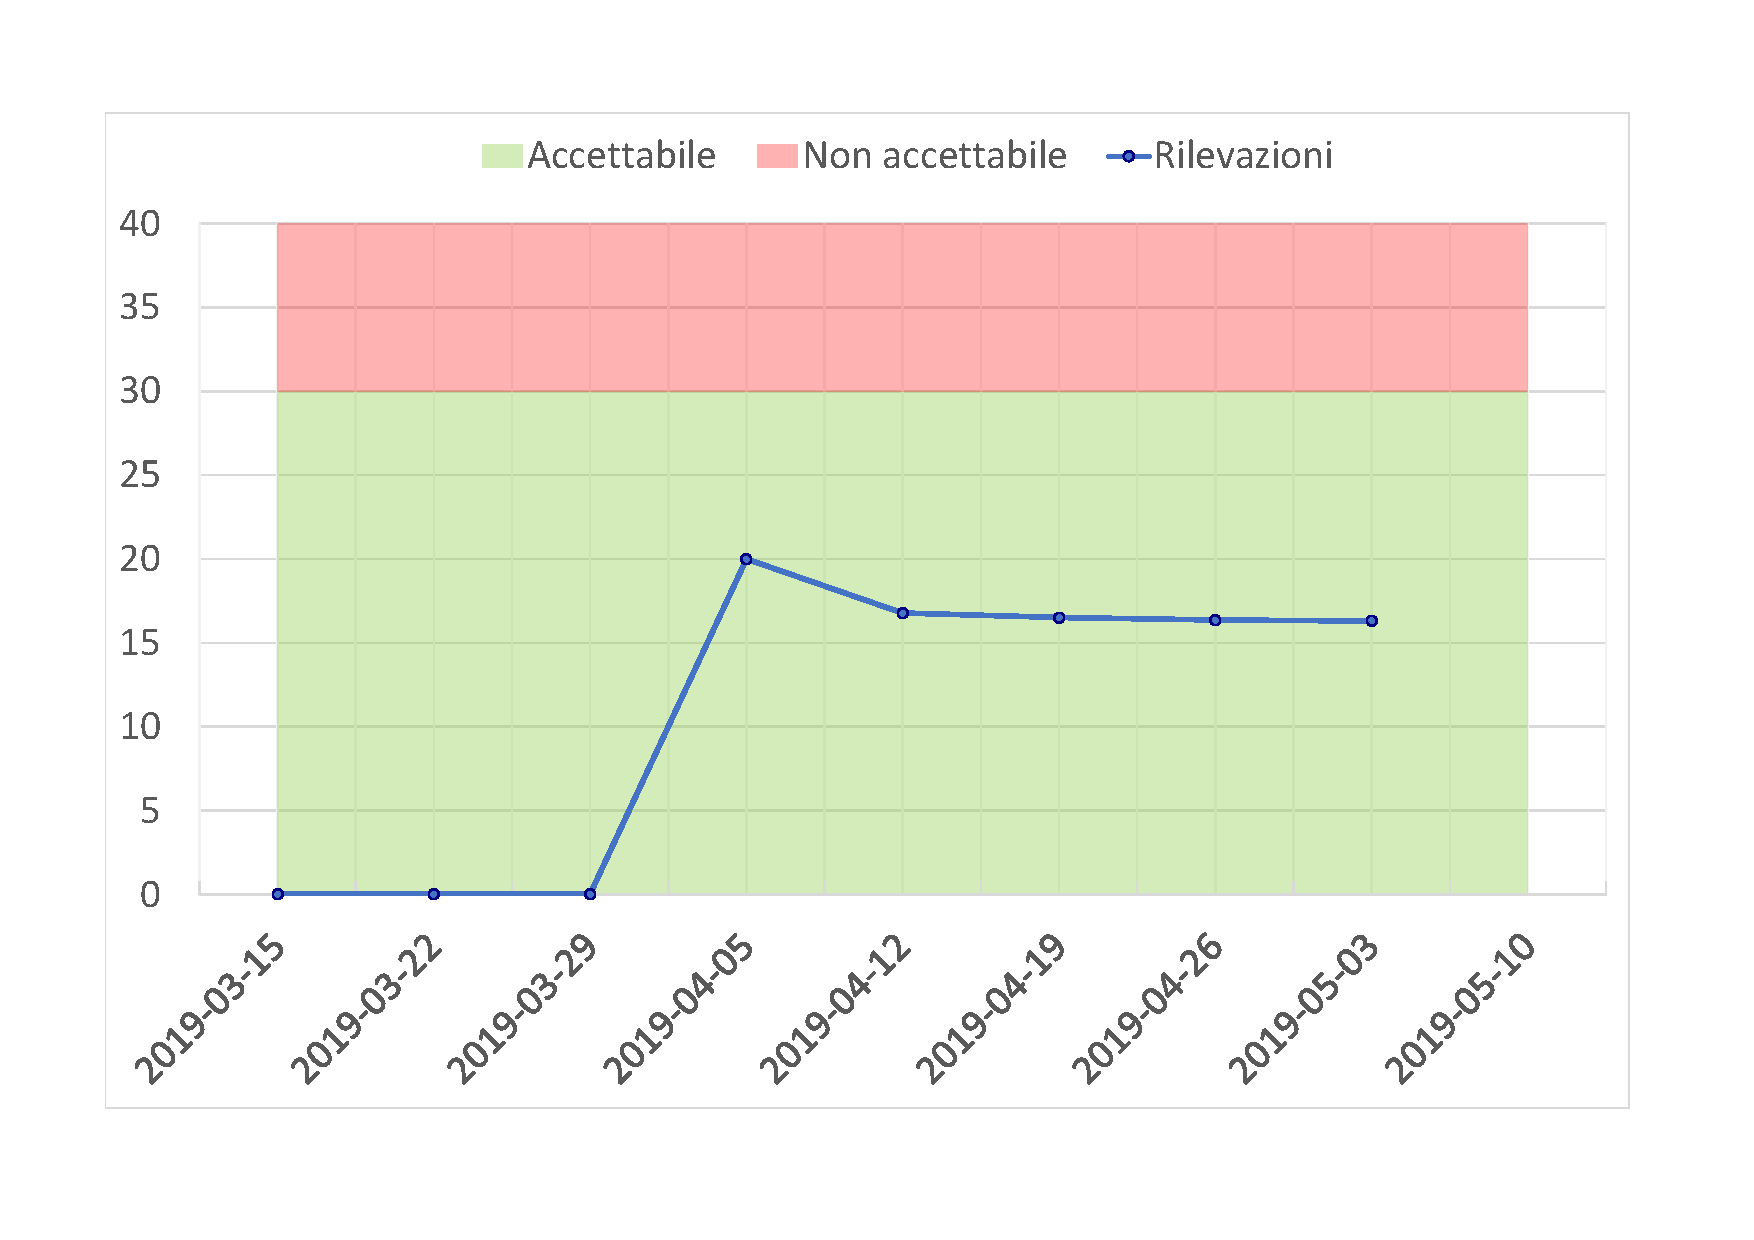
\includegraphics[scale=0.6]{images/resoconto/MPS10Chart.pdf}
	\caption{Serie storica linee di codice per procedura}	
\end{figure}

\subsection{Processi}
\subsubsection{Valori ISO/IEC 15504 - MPC1}

Riportiamo di seguito i grafici rappresentanti il livello raggiunto alla data di ogni revisione dai vari processi.


\begin{figure}[H]
	\centering
	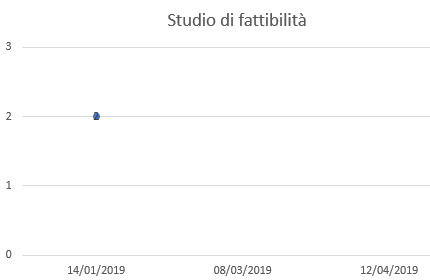
\includegraphics[scale=1]{images/resoconto/Studio.png}
	\caption{Valori ISO/IEC 15504 - Studio di fattibilità}	
\end{figure}


\begin{figure}[H]
	\centering
	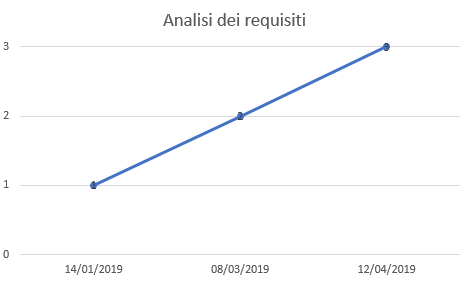
\includegraphics[scale=1]{images/resoconto/Analisi.png}
	\caption{Valori ISO/IEC 15504 - Analisi dei Requisiti}	
\end{figure}


\begin{figure}[H]
	\centering
	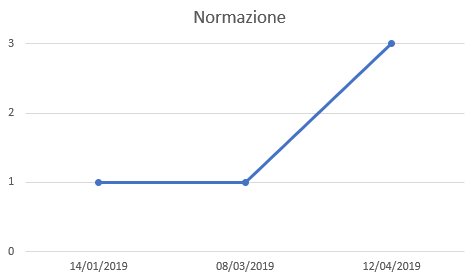
\includegraphics[scale=1]{images/resoconto/Normazione.png}
	\caption{Valori ISO/IEC 15504 - Normazione}	
\end{figure}


\begin{figure}[H]
	\centering
	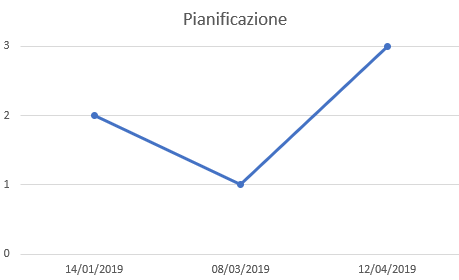
\includegraphics[scale=1]{images/resoconto/Pianificazione.png}
	\caption{Valori ISO/IEC 15504 - Pianificazione}	
\end{figure}


\begin{figure}[H]
	\centering
	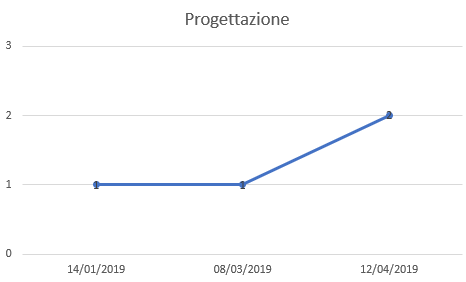
\includegraphics[scale=1]{images/resoconto/Progettazione.png}
	\caption{Valori ISO/IEC 15504 - Progettazione}	
\end{figure}


\begin{figure}[H]
	\centering
	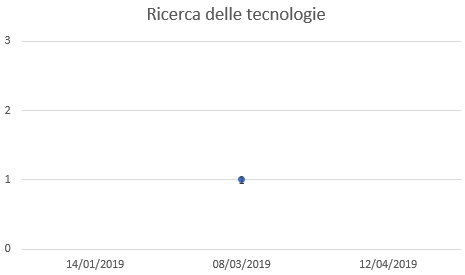
\includegraphics[scale=1]{images/resoconto/Ricerca.png}
	\caption{Valori ISO/IEC 15504 - Ricerca delle tecnologie}	
\end{figure}


\begin{figure}[H]
	\centering
	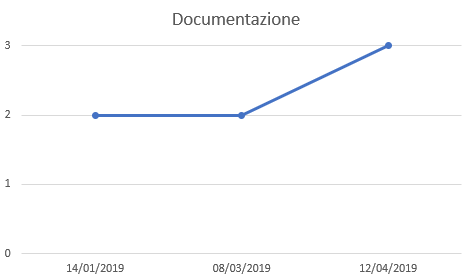
\includegraphics[scale=1]{images/resoconto/Documentazione.png}
	\caption{Valori ISO/IEC 15504 - Documentazione}	
\end{figure}


\begin{figure}[H]
	\centering
	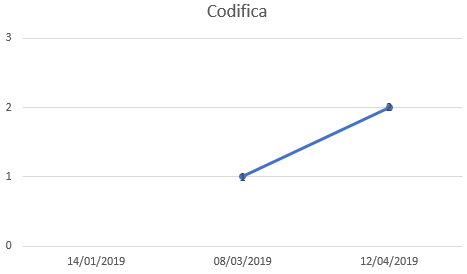
\includegraphics[scale=1]{images/resoconto/Codifica.png}
	\caption{Valori ISO/IEC 15504 - Codifica}	
\end{figure}
\newpage
\subsubsection{Valori indice RSI - MPC2\\}
Durante lo sviluppo del progetto abbiamo individuato periodicamente tutti i cambiamenti apportati ai requisiti del progetto. Questo ci ha permesso di determinare la stabilità dei requisiti nel tempo grazie all'utilizzo della metrica MPC2.
Riportiamo di seguito i calcoli e le varie rilevazioni effettuate.

\begin{longtable}{>{\centering\arraybackslash}m{3cm} >{\centering\arraybackslash}m{4cm} >{\centering\arraybackslash}m{5cm} >{\centering\arraybackslash}m{2cm}}
	\rowcolor{LightBlue}
	\textbf{\textcolor{white}{Data rilevazioni}}
	& \textbf{\textcolor{white}{Requirement Stability Index (RSI)}}
	& \textbf{\textcolor{white}{Esito}}\\
	
	2019-02-15 & \[1-\frac{0+5+4}{48}=0.81\] & Accettato\\
	\hline
	2019-02-20 & \[1-\frac{5+0+3}{43}=0.81\] & Accettato\\
	\hline
	2019-02-21 & \[1-\frac{8+0+3}{48}=0.77\] & Accettato\\
	\hline
	2019-02-22 & \[1-\frac{5+2+0}{56}=0.85\] & Accettato\\
	\hline
	2019-02-25 & \[1-\frac{11+0+0}{59}=0.81\] & Accettato\\
	\hline
	2019-02-27 & \[1-\frac{10+0+0}{70}=0.88\] & Accettato\\
	\hline
	2019-03-04 & \[1-\frac{12+0+0}{80}=0.86\] & Accettato\\
	\hline
	2019-03-05 & \[1-\frac{14+0+1}{92}=0.83\] & Accettato\\
	\hline\\
	\caption{Rilevazioni indice stabilità requisiti (RSI) - Revisione di progetto}
\end{longtable}

\begin{longtable}{>{\centering\arraybackslash}m{3cm} >{\centering\arraybackslash}m{4cm} >{\centering\arraybackslash}m{5cm} >{\centering\arraybackslash}m{2cm}}
	\rowcolor{LightBlue}
	\textbf{\textcolor{white}{Data rilevazioni}}
	& \textbf{\textcolor{white}{Requirement Stability Index (RSI)}}
	& \textbf{\textcolor{white}{Esito}}\\
	
	2019-03-18 & \[1-\frac{9+0+0}{106}=0.915\] & Accettato\\
	\hline
	2019-03-19 & \[1-\frac{13+0+2}{115}=0.87\] & Accettato\\
	\hline
	\caption{Rilevazioni indice stabilità requisiti (RSI) - Revisione di qualifica}
\end{longtable}

\begin{longtable}{>{\centering\arraybackslash}m{3cm} >{\centering\arraybackslash}m{4cm} >{\centering\arraybackslash}m{5cm} >{\centering\arraybackslash}m{2cm}}
	\rowcolor{LightBlue}
	\textbf{\textcolor{white}{Data rilevazioni}}
	& \textbf{\textcolor{white}{Requirement Stability Index (RSI)}}
	& \textbf{\textcolor{white}{Esito}}\\
	2019-04-30 & \[1-\frac{2+3+0}{128}=0.96\] & Accettato\\
	\hline
	2019-05-07 & \[1-\frac{0+2+0}{127}=0.98\] & Accettato\\
	\hline
	\caption{Rilevazioni indice stabilità requisiti (RSI) - Revisione di accettazione}
\end{longtable}

\begin{figure}[H]
	\centering
	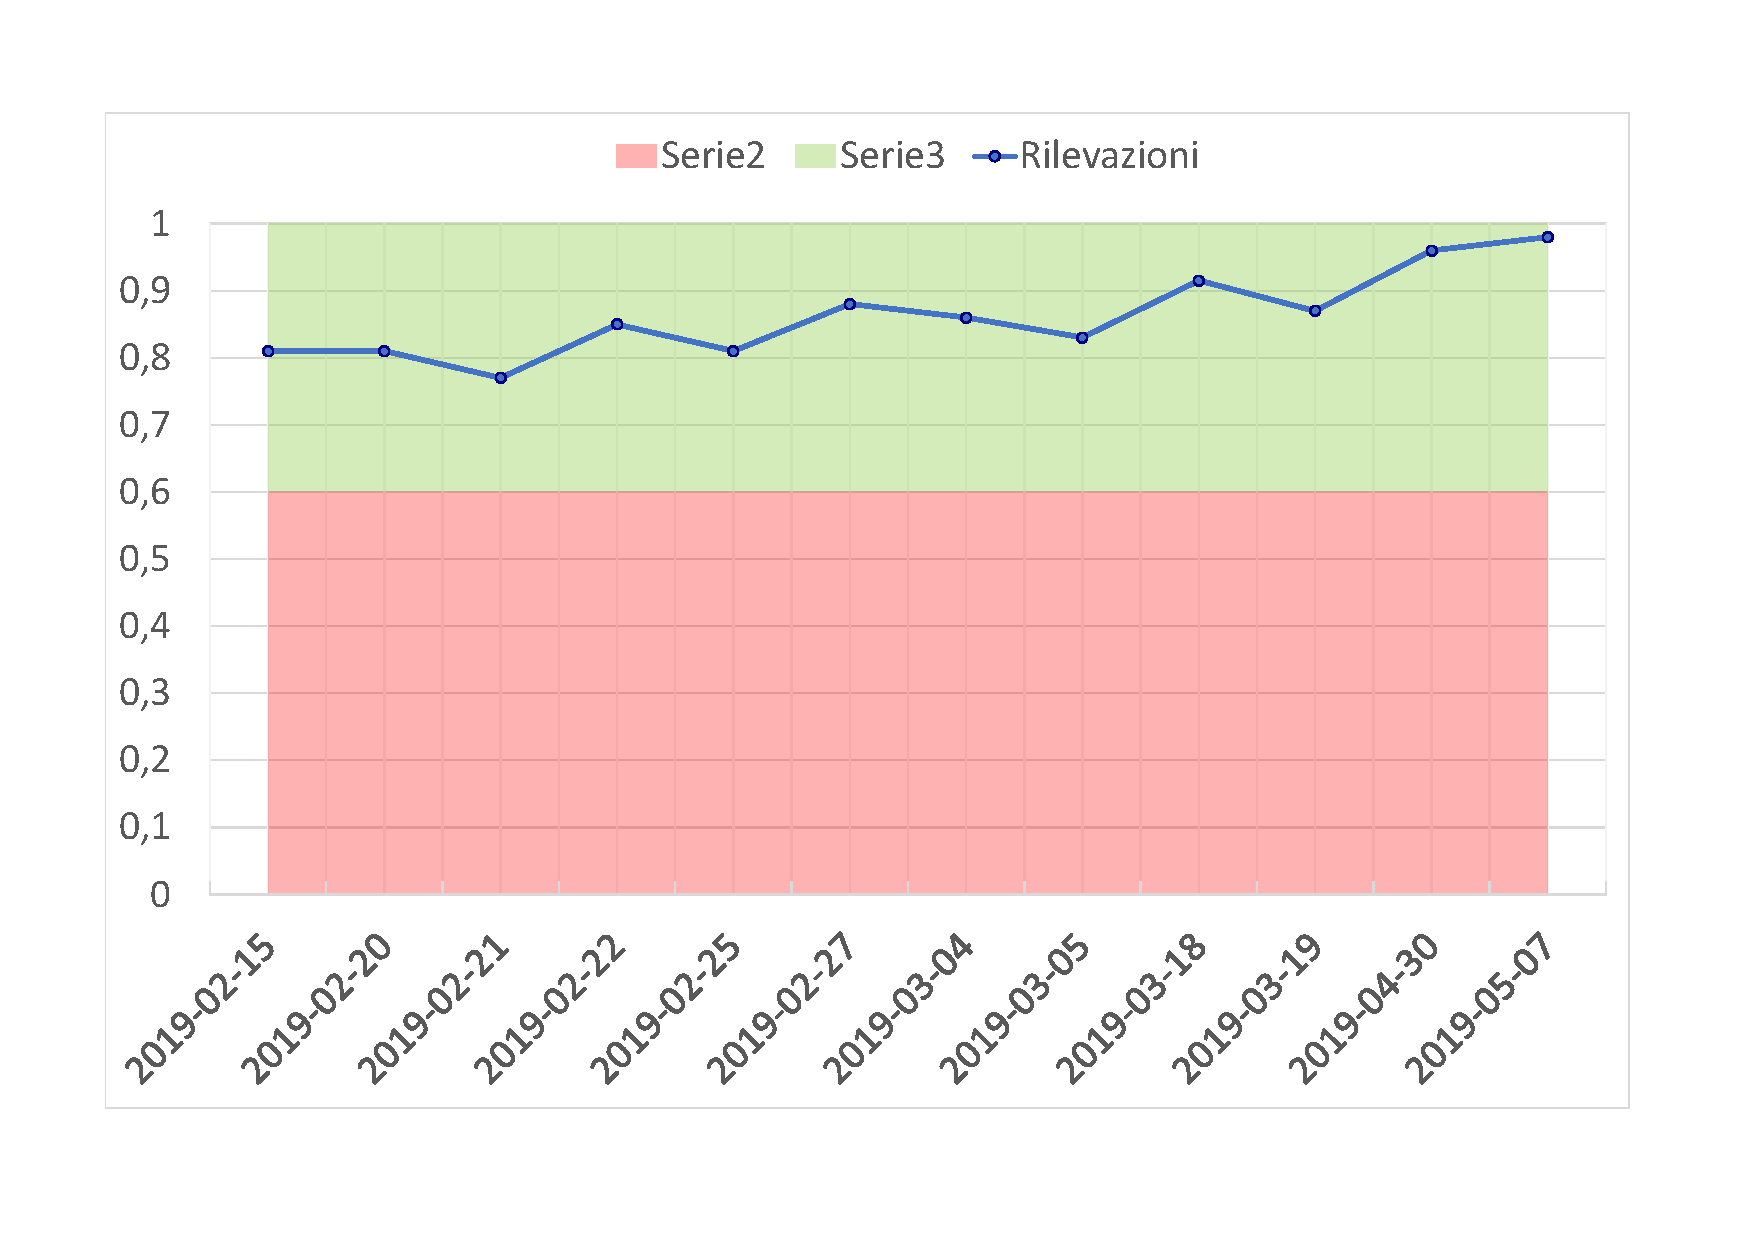
\includegraphics[scale=0.6]{images/resoconto/MPC2Chart.pdf}
	\caption{Serie storica rilevazioni stabilità requisiti}	
\end{figure}


\subsubsection{Violazione dello stile di codifica - MPC3}

\subparagraph{Codifica al 2019-04-05}
In questo periodo dell'attività di codifica, sono state commesse 20 violazioni dello stile di codifica, così distribuite:
 \begin{itemize}
 	\item \textbf{Utilizzo lingua inglese}: 13 violazioni.
 	\item \textbf{Utilizzo TSLint}: 0 violazioni.
 	\item \textbf{Lunghezza linee di codice}: 2 violazioni.
 	\item \textbf{Nomenclatura}: 0 violazioni.
 	\item \textbf{Commenti al codice}: 5 violazioni.
 \end{itemize}
Questi dati non sono accettabili, il gruppo si impegnerà a correggere le violazioni nel prossimo periodo di codifica.

\subparagraph{Codifica al 2019-04-12}
In questo periodo dell'attività di codifica, sono state commesse 7 violazioni dello stile di codifica, così distribuite:
 \begin{itemize}
 	\item \textbf{Utilizzo lingua inglese}: 0 violazioni.
 	\item \textbf{Utilizzo TSLint}: 0 violazioni.
 	\item \textbf{Lunghezza linee di codice}: 7 violazioni.
 	\item \textbf{Nomenclatura}: 0 violazioni.
 	\item \textbf{Commenti al codice}: 0 violazioni.
 \end{itemize}
Lo stile di codifica è migliorato rispetto alla precedente rilevazione. Tuttavia l'obbiettivo di avere un numero inferiore alle 10 violazioni è rispettato ma ancora migliorabile.

\subparagraph{Codifica al 2019-04-19}
In questo periodo dell'attività di codifica, sono state commesse 3 violazioni dello stile di codifica, così distribuite:
 \begin{itemize}
 	\item \textbf{Utilizzo lingua inglese}: 0 violazioni.
 	\item \textbf{Utilizzo TSLint}: 0 violazioni.
 	\item \textbf{Lunghezza linee di codice}: 3 violazioni.
 	\item \textbf{Nomenclatura}: 0 violazioni.
 	\item \textbf{Commenti al codice}: 0 violazioni.
 \end{itemize}
Lo stile di codifica è migliorato rispetto alla precedente rilevazione. Tuttavia l'obbiettivo di avere un numero inferiore alle 10 violazioni è rispettato ma ancora migliorabile.

\subparagraph{Codifica al 2019-04-26}
In questo periodo dell'attività di codifica, sono state commesse 6 violazioni dello stile di codifica, così distribuite:
 \begin{itemize}
 	\item \textbf{Utilizzo lingua inglese}: 0 violazioni.
 	\item \textbf{Utilizzo TSLint}: 0 violazioni.
 	\item \textbf{Lunghezza linee di codice}: 6 violazioni.
 	\item \textbf{Nomenclatura}: 0 violazioni.
 	\item \textbf{Commenti al codice}: 0 violazioni.
 \end{itemize}
Lo stile di codifica è migliorato rispetto alla precedente rilevazione. Tuttavia l'obbiettivo di avere un numero inferiore alle 10 violazioni è rispettato ma ancora migliorabile.

\subparagraph{Codifica al 2019-05-03}
In questo periodo dell'attività di codifica, sono state commesse 8 violazioni dello stile di codifica, così distribuite:
 \begin{itemize}
 	\item \textbf{Utilizzo lingua inglese}: 0 violazioni.
 	\item \textbf{Utilizzo TSLint}: 3 violazioni.
 	\item \textbf{Lunghezza linee di codice}: 5 violazioni.
 	\item \textbf{Nomenclatura}: 0 violazioni.
 	\item \textbf{Commenti al codice}: 0 violazioni.
 \end{itemize}
Lo stile di codifica è migliorato rispetto alla precedente rilevazione. Tuttavia l'obbiettivo di avere un numero inferiore alle 10 violazioni è rispettato.

\subparagraph{Codifica al 2019-05-10}
In questo periodo non si è verificata l'attività di codifica in quanto il prodotto è stato ritenuto concluso precedentemente.

\begin{figure}[H]
	\centering
	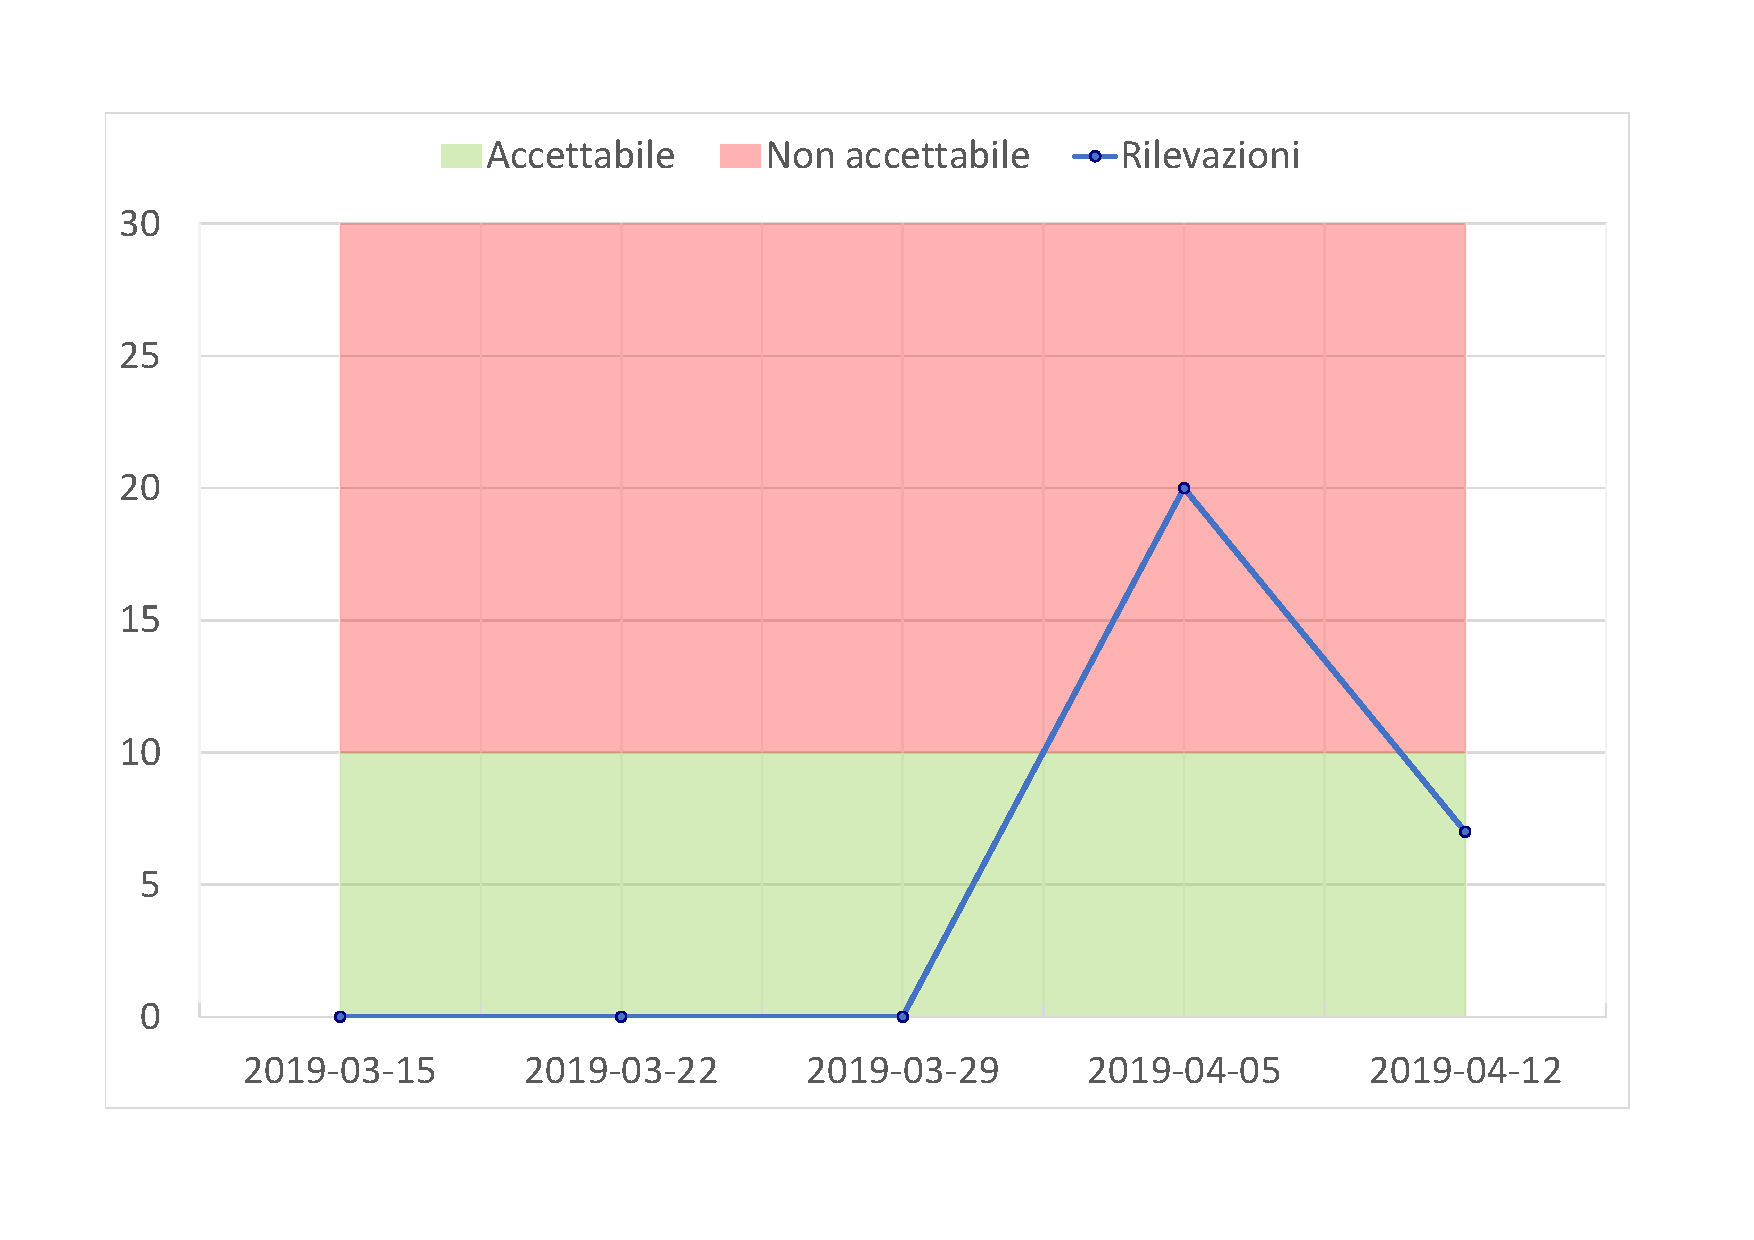
\includegraphics[scale=0.6]{images/resoconto/MPC3Chart.pdf}
	\caption{Serie storica numero di violazioni dello stile di codifica}	
\end{figure}

\subsubsection{Test di integrazione implementati - MPC4}
\subparagraph{Codifica al 2019-04-05}
In questo periodo dell'attività di codifica, è stato implementato 1 test di integrazione su un totale di 10 test di integrazione preventivati.
Nonostante non raggiunga il livello di accettazione della
metrica, questo risultato è ritenuto sufficiente a questo punto del progetto poiché sono previsti altri incrementi alla codifica che porteranno all'implementazione di altri test.

\subparagraph{Codifica al 2019-04-12}
In questo periodo dell'attività di codifica, sono stati implementati 3 test di integrazione per un totale di 4 coprendo il 40\% dei test di integrazione preventivati.
Nonostante non raggiunga il livello di accettazione della
metrica, questo risultato è ritenuto sufficiente a questo punto del progetto poiché sono previsti altri incrementi alla codifica che porteranno all'implementazione di altri test. 

\subparagraph{Codifica al 2019-04-19}
In questo periodo dell'attività di codifica, sono stati implementati 2 test di integrazione per un totale di 6 coprendo il 60\% dei test di integrazione preventivati.
Nonostante non raggiunga il livello di accettazione della
metrica, questo risultato è ritenuto sufficiente a questo punto del progetto poiché sono previsti altri incrementi alla codifica che porteranno all'implementazione di altri test. 

\subparagraph{Codifica al 2019-04-26}
In questo periodo dell'attività di codifica, sono stati implementati 2 test di integrazione per un totale di 8 coprendo il 80\% dei test di integrazione preventivati.
Nonostante non raggiunga il livello di accettazione della
metrica, questo risultato è ritenuto sufficiente a questo punto del progetto poiché sono previsti altri incrementi alla codifica che porteranno all'implementazione di altri test. 

\subparagraph{Codifica al 2019-05-03}
In questo periodo dell'attività di codifica, sono stati implementati 3 test di integrazione per un totale di 9 coprendo il 90\% dei test di integrazione preventivati.
A seguito di questo periodo di codifica la soglia di accettabilità della metrica è stata raggiunta.
Il gruppo si impegnerà ad implementare ulteriori test di integrazione.


\subparagraph{Codifica al 2019-05-10}
In questo periodo dell'attività di codifica, sono stati implementati 1 test di integrazione per un totale di 10 coprendo il 100\% dei test di integrazione preventivati.

\\
Riportiamo di seguito una tabella rappresentativa dello stato di avanzamento dei test. La tabella verrà aggiornata alla fine di ogni periodo dell'attività di codifica.

	\begin{longtable}{|>{\centering\arraybackslash}m{1.6cm}|>{\centering\arraybackslash}m{6.41cm}|>{\centering\arraybackslash}m{3.1cm}|}		
	\rowcolor{LightBlue}
	\textbf{\textcolor{white}{Test}}
	& \textbf{\textcolor{white}{Stato}}\\
	\hline
	TI1
	& Non implementato
	\\ \hline
	\rowcolor{LightGray}
	TI2
	& Non implementato
	\\ \hline
	TI3
	& Non implementato
	\\ \hline
	\rowcolor{LightGray}
	TI4
	& Non implementato
	\\ \hline
	TI5
	& Non implementato
	\\ \hline
	\rowcolor{LightGray}
	TI6
	& Non implementato
	\\ \hline	
	TI7
	& Implementato
	\\ \hline	
	\rowcolor{LightGray}
	TI8
	& Implementato
	\\ \hline	
	TI9
	& Implementato
	\\ \hline	
	\rowcolor{LightGray}
	TI10
	& Implementato
	\\ \hline	
	\caption{Test di integrazione - stato di avanzamento}
\end{longtable}

\begin{figure}[H]
	\centering
	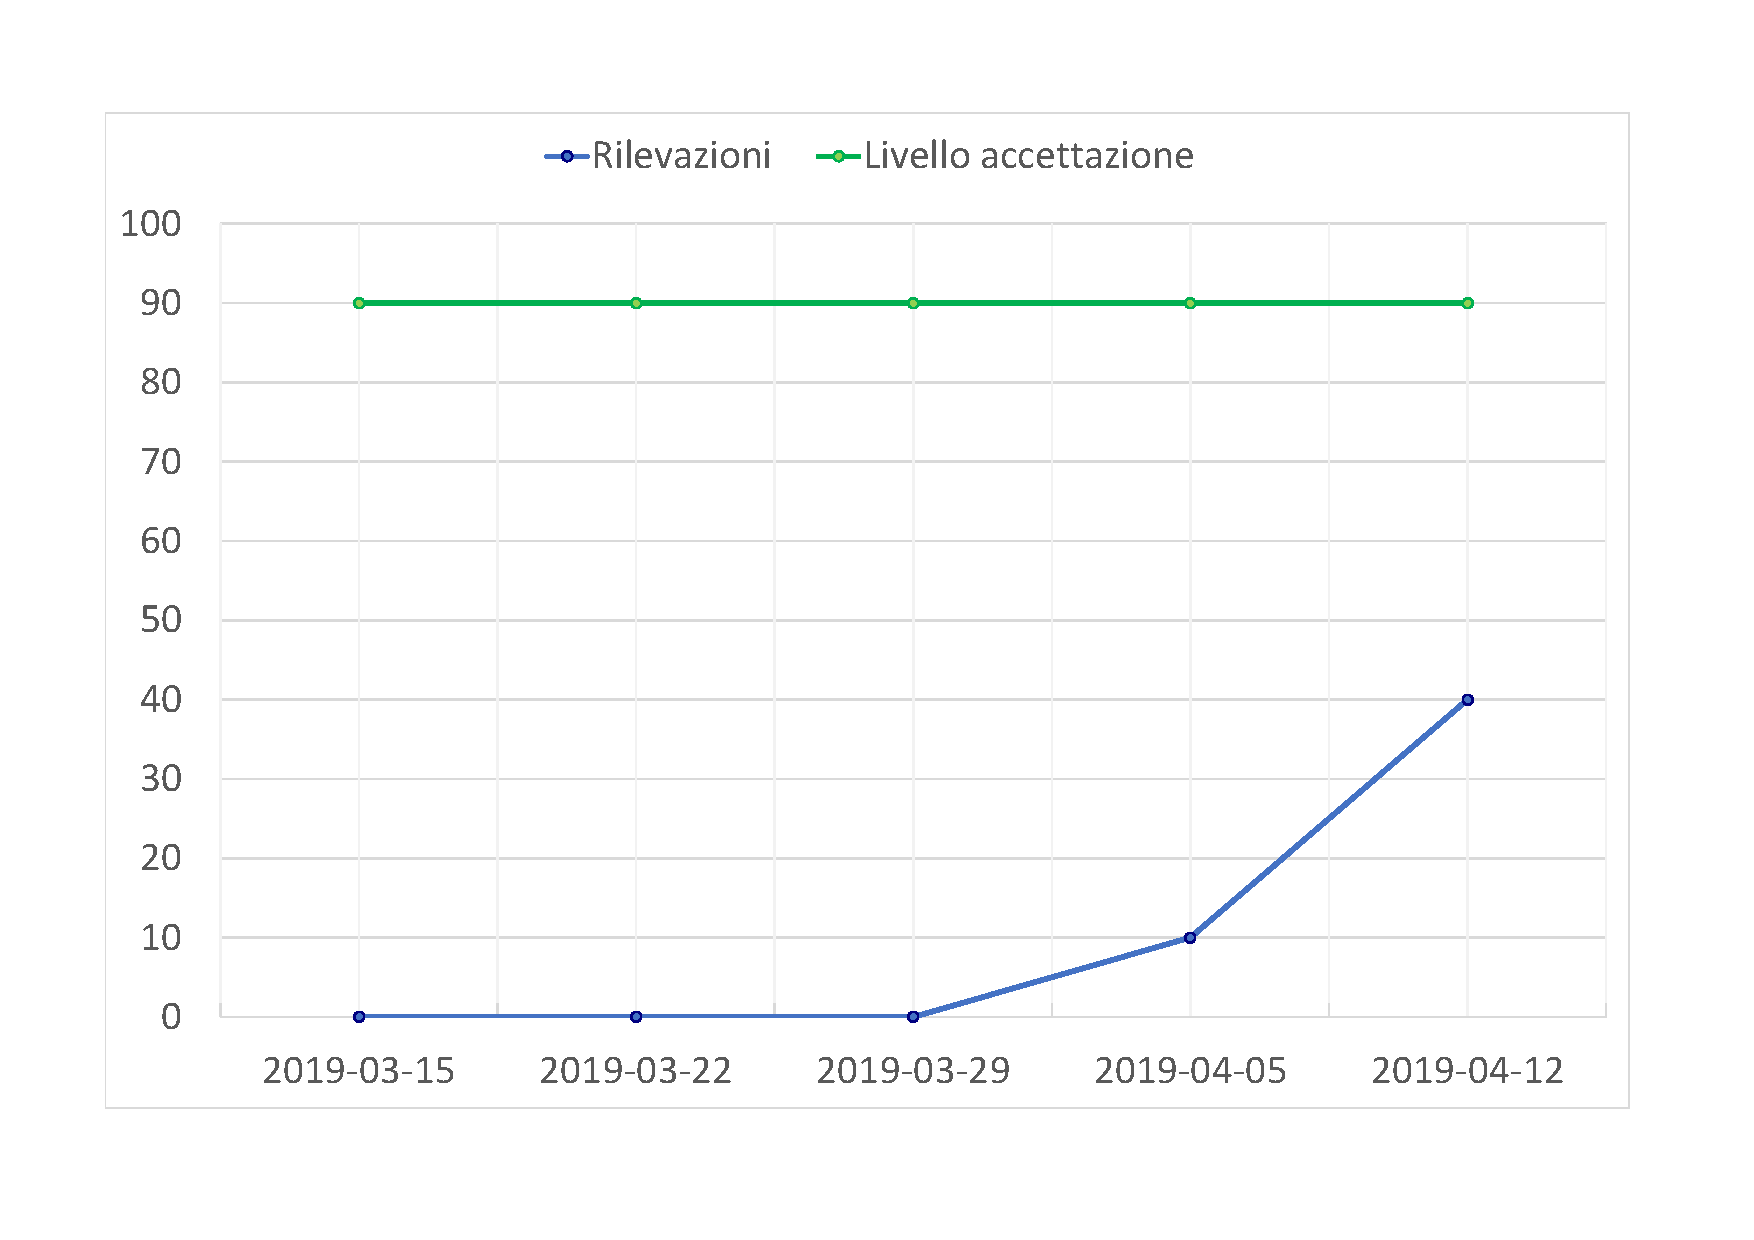
\includegraphics[scale=0.6]{images/resoconto/MPC4Chart.pdf}
	\caption{Serie storica linee di codice per procedura}	
\end{figure}

\subsubsection{Test di sistema implementati - MPC5}
\subparagraph{Codifica al 2019-04-19}


\subparagraph{Codifica al 2019-04-26}


\subparagraph{Codifica al 2019-05-03}


\subparagraph{Codifica al 2019-05-10}




%TODO
\subsubsection{Test di unità implementati - MPC6}
\subparagraph{Codifica al 2019-04-05}
In questo periodo dell'attività di codifica, è stato implementato 20 test di unità su un totale di 134 coprendo il \% dei test di unità preventivati.
Nonostante non raggiunga il livello di accettazione della
metrica, questo risultato è ritenuto sufficiente a questo punto del progetto poiché sono previsti altri incrementi alla codifica che porteranno all'implementazione di altri test.

\subparagraph{Codifica al 2019-04-12}
In questo periodo dell'attività di codifica, sono stati implementati 18 test di unità per un totale di 38 coprendo il \% dei test di unità preventivati.
Nonostante non raggiunga il livello di accettazione della
metrica, questo risultato è ritenuto sufficiente a questo punto del progetto poiché sono previsti altri incrementi alla codifica che porteranno all'implementazione di altri test.

\subparagraph{Codifica al 2019-04-19}
In questo periodo dell'attività di codifica, sono stati implementati 30 test di unità per un totale di 68 coprendo il \% dei test di unità preventivati.
Nonostante non raggiunga il livello di accettazione della
metrica, questo risultato è ritenuto sufficiente a questo punto del progetto poiché sono previsti altri incrementi alla codifica che porteranno all'implementazione di altri test.

\subparagraph{Codifica al 2019-04-26}
In questo periodo dell'attività di codifica, sono stati implementati 38 test di unità per un totale di 106 coprendo il \% dei test di unità preventivati.
Nonostante non raggiunga il livello di accettazione della
metrica, questo risultato è ritenuto sufficiente a questo punto del progetto poiché sono previsti altri incrementi alla codifica che porteranno all'implementazione di altri test.

\subparagraph{Codifica al 2019-05-03}
In questo periodo dell'attività di codifica, sono stati implementati 28 test di unità per un totale di 134 coprendo il \% dei test di unità preventivati.
Nonostante non raggiunga il livello di accettazione della
metrica, questo risultato è ritenuto sufficiente a questo punto del progetto poiché sono previsti altri incrementi alla codifica che porteranno all'implementazione di altri test.

\subparagraph{Codifica al 2019-05-10}
In questo periodo dell'attività di codifica, sono stati implementati  test di unità per un totale di  coprendo il \% dei test di unità preventivati.
Nonostante non raggiunga il livello di accettazione della
metrica, questo risultato è ritenuto sufficiente a questo punto del progetto poiché sono previsti altri incrementi alla codifica che porteranno all'implementazione di altri test.
\\Riportiamo di seguito una tabella rappresentativa dello stato di avanzamento dei test. La tabella verrà aggiornata alla fine di ogni periodo dell'attività di codifica.

\begin{longtable}{|>{\centering\arraybackslash}m{1.6cm}|>{\centering\arraybackslash}m{6.41cm}|>{\centering\arraybackslash}m{3.1cm}| c |}		
	\rowcolor{LightBlue}
	\textbf{\textcolor{white}{Test}}
	& \textbf{\textcolor{white}{Stato}}
	& \textbf{\textcolor{white}{Esito}}\\
	\hline
	TU1 & Implementato & Superato \\ \hline
	TU2 & Implementato & Superato  \\ \hline
	TU3 & Implementato & Superato  \\ \hline
	TU4 & Implementato & Superato  \\ \hline
	TU5 & Implementato & Superato  \\ \hline
	TU6 & Implementato & Superato  \\ \hline
	TU7 & Implementato & Superato  \\ \hline
	TU8 & Implementato & Superato  \\ \hline
	TU9 & Implementato & Superato  \\ \hline
	TU10 & Implementato & Superato  \\ \hline
	TU11 & Implementato & Superato  \\ \hline		
	TU12 & Implementato & Superato  \\ \hline
	TU13 & Implementato & Superato  \\ \hline
	TU14 & Implementato & Superato \\ \hline
	TU15 & Implementato & Superato  \\ \hline
	TU16 & Implementato & Superato \\ \hline
	TU17 & Implementato & Superato \\ \hline
	TU18 & Implementato & Superato \\ \hline
	TU19 & Implementato & Superato \\ \hline
	TU20 & Implementato & Superato \\ \hline
	TU21 & Implementato & Superato \\ \hline
	TU22 & Implementato & Superato \\ \hline
	TU23 & Implementato & Superato \\ \hline
	TU24 & Implementato & Superato \\ \hline
	TU25 & Implementato & Superato \\ \hline		
	TU26 & Implementato & Superato \\ \hline
	TU27 & Implementato & Superato  \\ \hline
	TU28 & Implementato & Superato  \\ \hline
	TU29 & Implementato & Superato  \\ \hline
	TU30 & Implementato & Superato  \\ \hline
	TU31 & Implementato & Superato  \\ \hline
	TU32 & Implementato & Superato  \\ \hline
	TU33 & Implementato & Superato  \\ \hline
	TU34 & Implementato & Superato  \\ \hline
	TU35 & Implementato & Superato \\ \hline
	TU36 & Implementato & Superato \\ \hline
	TU37 & Implementato & Superato  \\ \hline
	TU38 & Implementato & Superato  \\ \hline
	TU39 & Non implementato & Non superato \\ \hline
	TU40 & Non implementato & Non superato \\ \hline
	TU41 & Non implementato & Non superato \\ \hline
	TU42 & Non implementato & Non superato \\ \hline
	TU43 & Non implementato & Non superato \\ \hline
	TU44 & Non implementato & Non superato \\ \hline
	TU45 & Non implementato & Non superato \\ \hline
	TU46 & Non implementato & Non superato \\ \hline
	TU47 & Non implementato & Non superato \\ \hline
	TU48 & Non implementato & Non superato \\ \hline
	\caption{Test di unità - stato di avanzamento}
\end{longtable}

\begin{figure}[H]
	\centering
	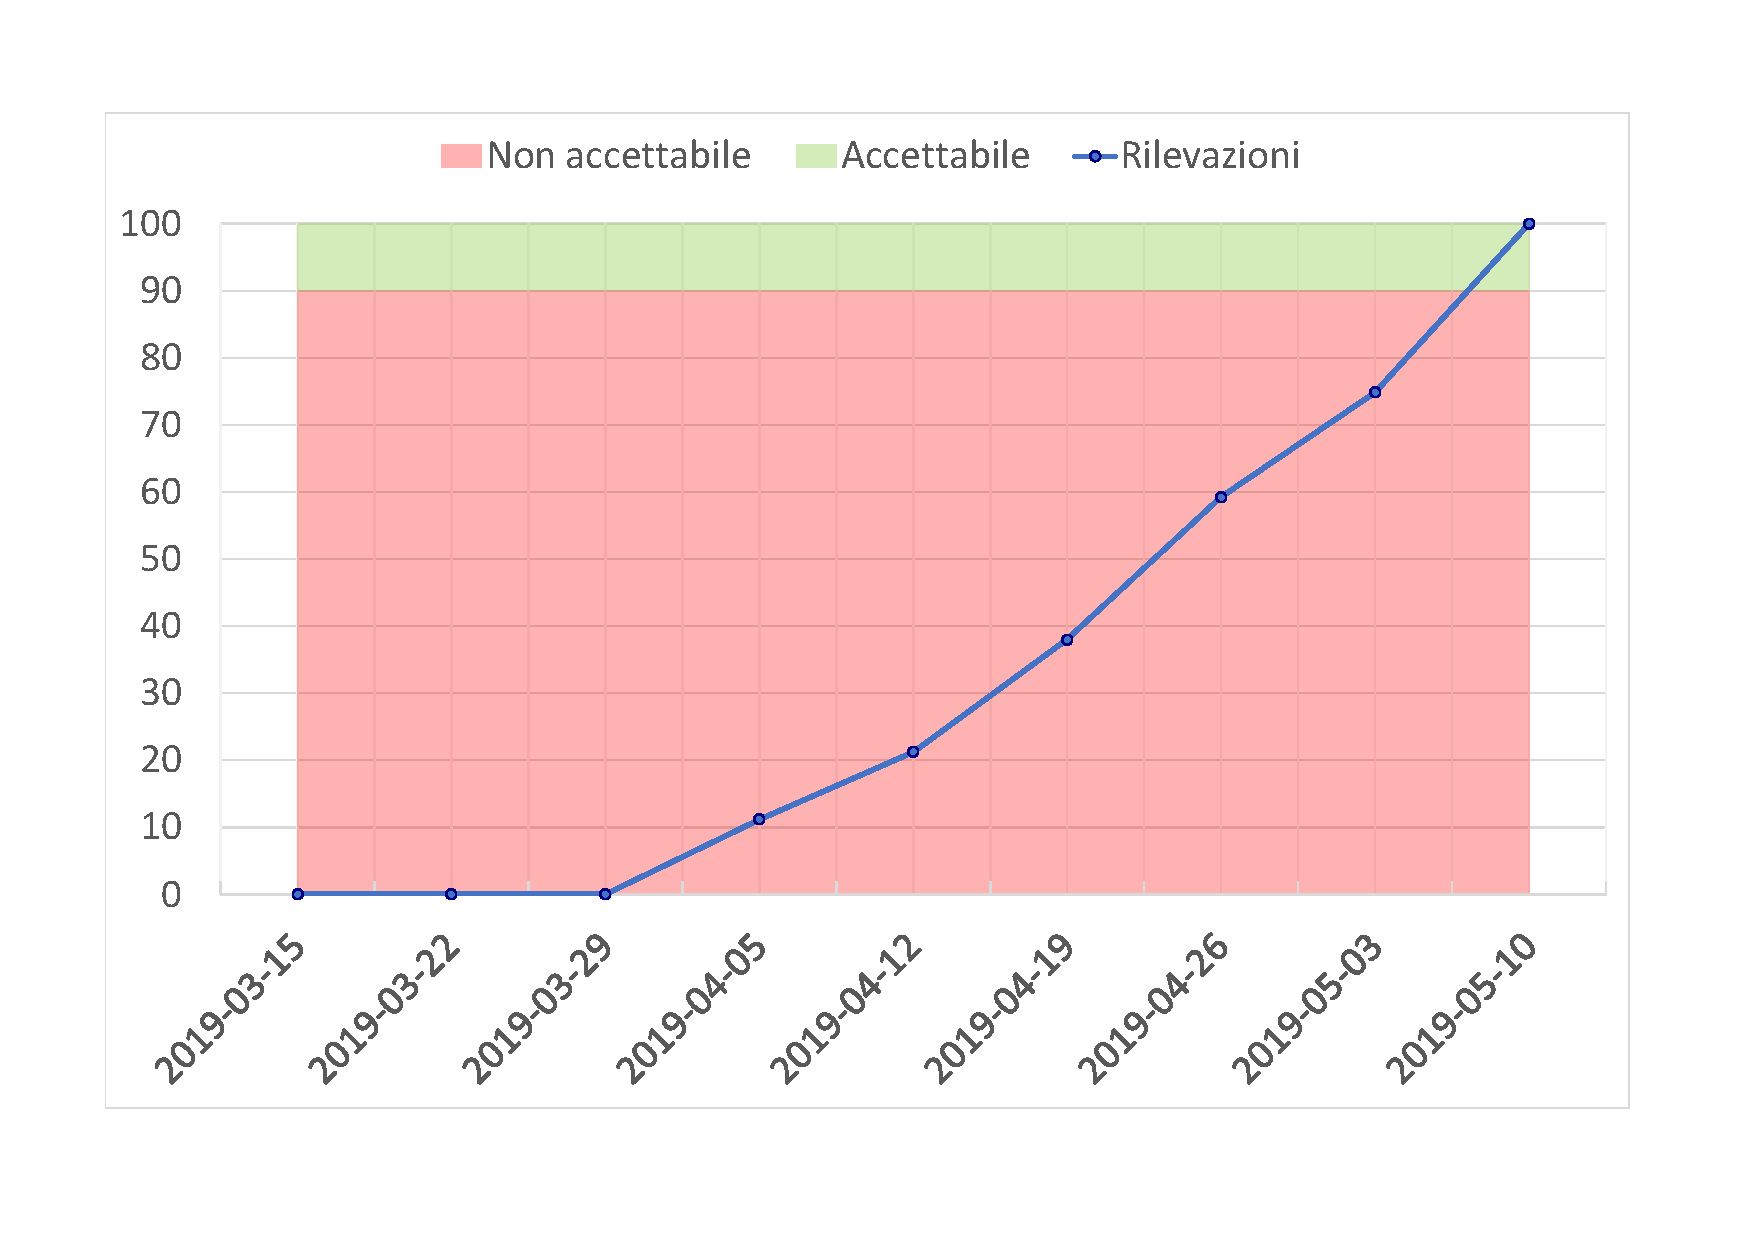
\includegraphics[scale=0.6]{images/resoconto/MPC6Chart.pdf}
	\caption{Serie storica test di unità implementati}	
\end{figure}

\subsubsection{Test di accettazione implementati - MPC7}
In questa fase non sono stati implementati test di accettazione.
Il gruppo si impegnerà all'implementazione degli stessi nella prossima fase.
\newpage
\subsection{Esito delle revisioni - RR}
Successivamente alla prima revisione formale, il gruppo ha apportato diverse modifiche ai documenti basandosi sulle osservazioni ricevute dai docenti. Le modifiche sono riassunte di seguito:
	\begin{itemize}
		\item \textbf{Norme di Progetto}: è stata aggiunta una sezione riportante le metriche di riferimento per processi e prodotti e la relativa normazione. 
		\item \textbf{Piano di Progetto}: le attività sono state ripianificate a partire dalla fase 2 ed è stato redatto un nuovo consuntivo.
		\item \textbf{Piano di Qualifica}: la struttura del documento è stata completamente rivista, i contenuti sono stati modificati secondo le indicazioni riportate nell'esito della prima revisione. Sono stati aggiunti diversi tipi di test e diverse appendici con argomenti vari; sono stati stabiliti degli obiettivi di qualità.
		\item \textbf{Analisi dei Requisiti}: sono stati aggiunti diversi nuovi casi d'uso, specializzando quelli già presenti e raddoppiandone il numero; sono stati modificati i diagrammi UML. \`E stata aggiunta una sezione introduttiva ed una descrizione degli attori implicati nel progetto. 
	\end{itemize}

\subsection{Esito delle revisioni - RP}	
Successivamente alla seconda revisione formale, il gruppo ha apportato diverse modifiche ai documenti basandosi sulle osservazioni ricevute dai docenti. Le modifiche sono riassunte di seguito:
	\begin{itemize}
		\item \textbf{Norme di Progetto}: sono state aggiunte diverse norme ed attività al processo di fornitura, revisionando contestualmente quelle già inserite. Sono state rimosse le soglie associate ad ogni metrica e la struttura del documento è stata in parte rivisitata.
		\item \textbf{Piano di Progetto}: le fasi 3 e 4 sono state ripianificate sulla base del periodo precedente; si è cercato di dare maggiore spessore all'incrementalità della logica di sviluppo adottata. 
		\item \textbf{Piano di Qualifica}: la struttura del documento è stata revisionata, sono stati redatti i test di unità e si è cercato di dare una struttura a cruscotto ai riscontri di verifica.
		\item \textbf{Analisi dei Requisiti}: i casi d'uso sono stati rivisti, aumentandone quanto possibile il livello di dettaglio; i codici dei casi d'uso e dei requisiti sono stati modificati e, di conseguenza, hanno subito modifiche anche i diagrammi UML.
	\end{itemize}

\subsection{Esito delle revisioni - RQ}	
Successivamente alla terza revisione formale, il gruppo ha apportato diverse modifiche ai documenti basandosi sulle osservazioni ricevute dai docenti. Le modifiche sono riassunte di seguito:
	\begin{itemize}
		\item \textbf{Norme di Progetto}: 
		\item \textbf{Piano di Progetto}: non sono state apportate modifiche rilevanti al documento
		\item \textbf{Piano di Qualifica}: sono stati aggiornati gli elenchi dei test applicati al sistema (di unità, integrazione, sistema e validazione) e la lista dei requisiti soddisfatti. 
		\item \textbf{Analisi dei Requisiti}: sono stati modificati i diagrammi UML per i casi UC-M1.3, UC-M3 e UC-I10.1, secondo le segnalazioni ricevute.
		\item \textbf{Manuale Utente}: sono stati riportati i requisiti hardware come segnalato ed il documento è stato completato.
		\item \textbf{Manuale Sviluppatore}: il documento è stato modificato secondo indicazioni ed i temi sono stati approfonditi in alcuni punti; il documento è stato poi completato.
	\end{itemize}
\newpage
\section{Copertura dei requisiti}
Viene riportata in seguito una tabella riassuntiva dei requisiti che non è da considerarsi definitiva, verrà infatti aggiornata in seguito ad ogni avanzamento significativo. \\
I requisiti sono indicati con il loro codice identificativo definito nel documento \textit{NormeDiProgetto\_v3.0.0} e la loro descrizione dettagliata è riportata nel documento \textit{AnalisiDeiRequisiti\_v3.0.0}.
\begin{longtable}{| p{2.5cm} | p{3cm} |}
	\rowcolor{LightBlue}
	\color{white}\bfseries Requisito & \color{white}\bfseries Stato \\
	ROF1 & Soddisfatto \\ \hline
	ROF2 & Soddisfatto \\ \hline
	ROF3 & Soddisfatto \\ \hline
	ROF4 & Soddisfatto \\ \hline
	ROF5 & Soddisfatto \\ \hline
	ROF6 & Soddisfatto \\ \hline
	ROF7 & Soddisfatto \\ \hline
	ROF8 & Soddisfatto \\ \hline
	ROF9 & Soddisfatto \\ \hline
	ROF10 & Soddisfatto \\ \hline
	ROF11 & Soddisfatto \\ \hline
	ROF12 & Soddisfatto \\ \hline
	ROF13 & Soddisfatto \\ \hline
	ROF14 & Soddisfatto \\ \hline
	ROF15 & Soddisfatto \\ \hline
	ROF16 & Soddisfatto \\ \hline
	ROF17 & Soddisfatto \\ \hline
	ROF18 & Soddisfatto \\ \hline
	ROF19 & Soddisfatto \\ \hline
	ROF20 & Soddisfatto \\ \hline
	ROF21 & Soddisfatto \\ \hline
	ROF22 & Soddisfatto \\ \hline
	ROF23 & Soddisfatto \\ \hline
	ROF24 & Soddisfatto \\ \hline
	ROF25 & Soddisfatto \\ \hline
	ROF26 & Soddisfatto \\ \hline
	ROF27 & Soddisfatto \\ \hline
	ROF28 & Soddisfatto \\ \hline
	ROF29 & Soddisfatto \\ \hline
	ROF30 & Soddisfatto \\ \hline
	ROF31 & Soddisfatto \\ \hline
	ROF32 & Soddisfatto \\ \hline
	ROF33 & Soddisfatto \\ \hline
	ROF34 & Soddisfatto \\ \hline
	ROF35 & Soddisfatto \\ \hline
	ROF36 & Soddisfatto \\ \hline
	ROF37 & Soddisfatto \\ \hline
	ROF38 & Soddisfatto \\ \hline
	ROF39 & Soddisfatto \\ \hline
	RDF1 & Soddisfatto \\ \hline
	RDF2 & Soddisfatto \\ \hline
	RDF3 & Soddisfatto \\ \hline
	RDF4 & Soddisfatto \\ \hline
	RDF5 & Soddisfatto \\ \hline
	RDF6 & Soddisfatto \\ \hline
	RDF7 & Soddisfatto \\ \hline
	RDF8 & Soddisfatto \\ \hline
	RDF9 & Soddisfatto \\ \hline
	RDF10 & Non soddisfatto \\ \hline
	RDF11 & Non soddisfatto \\ \hline
	RDF12 & Non soddisfatto \\ \hline
	RDF13 & Non soddisfatto \\ \hline
	RDF14 & Non soddisfatto \\ \hline
	RDF15 & Non soddisfatto \\ \hline
	RDF16 & Non soddisfatto \\ \hline
	RDF17 & Non soddisfatto \\ \hline
	RDF18 & Non soddisfatto \\ \hline
	RDF19 & Soddisfatto \\ \hline
	RDF20 & Non soddisfatto \\ \hline
	RDF21 & Non soddisfatto \\ \hline
	RDF22 & Soddisfatto\\ \hline
	RDF23 & Soddisfatto \\ \hline
	RDF24 & Soddisfatto \\ \hline
	RDF25 & Soddisfatto\\ \hline
	RDF26 & Non soddisfatto\\ \hline
	RDF27 & Non soddisfatto\\ \hline
	RDF28 & Soddisfatto \\ \hline
	RDF29 & Soddisfatto \\ \hline
	RDF30 & Soddisfatto \\ \hline
	RDF31 & Soddisfatto \\ \hline
	RDF32 & Soddisfatto \\ \hline
	RDF33 & Non soddisfatto\\ \hline
	RDF34 & Non soddisfatto \\ \hline
	RDF35 & Soddisfatto \\ \hline
	RDF36 & Non soddisfatto \\ \hline
	RDF37 & Non soddisfatto \\ \hline
	RDF38 & Soddisfatto \\ \hline
	RDF39 & Non soddisfatto \\ \hline
	RDF40 & Non soddisfatto \\ \hline
	RDF41 & Non soddisfatto \\ \hline
	RDF42 & Non soddisfatto \\ \hline
	RDF43 & Non soddisfatto \\ \hline
	RPF1 & Non soddisfatto \\ \hline
	RPF2 & Non soddisfatto \\ \hline
	RPF3 & Non soddisfatto \\ \hline
	RPF4 & Non soddisfatto \\ \hline
	RPF5 & Non soddisfatto \\ \hline
	RPF6 & Non soddisfatto \\ \hline
	RPF7 & Non soddisfatto \\ \hline
	RPF8 & Non soddisfatto \\ \hline
	RPF9 & Non soddisfatto \\ \hline
	RPF10 & Non soddisfatto \\ \hline
	RPF11 & Non soddisfatto \\ \hline
	RPF12 & Non soddisfatto \\ \hline
	RPF13 & Soddisfatto \\ \hline
	RPF14 & Non soddisfatto \\ \hline
	RPF15 & Soddisfatto \\ \hline
	RPF16 & Soddisfatto \\ \hline
	RPF17 & Non soddisfatto \\ \hline
	RPF18 & Non soddisfatto \\ \hline
	RPF19 & Non soddisfatto \\ \hline
	RPF20 & Soddisfatto \\ \hline
	RPF21 & Non soddisfatto \\ \hline
	RPF22 & Soddisfatto \\ \hline
	RPF23 & Non soddisfatto \\ \hline
	RPF24 & Non soddisfatto \\ \hline
	RPF25 & Non soddisfatto \\ \hline
	RPF26 & Non soddisfatto \\ \hline
	RPF27 & Soddisfatto \\ \hline
	RPF28 & Non soddisfatto \\ \hline
	RPF29 & Non soddisfatto \\ \hline
	RPF30 & Non soddisfatto \\ \hline
	ROV1 & Soddisfatto \\ \hline
	ROV2 & Soddisfatto \\ \hline
	ROV3 & Soddisfatto \\ \hline
	ROV4 & Soddisfatto \\ \hline
	RDV1 & Soddisfatto \\ \hline
	RPV1 & Non soddisfatto \\ \hline
	ROQ1 & Soddisfatto \\ \hline
	ROQ2 & Soddisfatto \\ \hline
	ROQ3 & Soddisfatto \\ \hline
	RDQ1 & Soddisfatto \\ \hline
	RDQ2 & Non soddisfatto \\ \hline
	RDQ3 & Soddisfatto \\ \hline
	RDQ4 & Non soddisfatto \\ \hline
	RDQ5 & Soddisfatto \\ \hline
	RPQ1 & Non soddisfatto \\ \hline
	\caption{Riassunto copertura requisiti}
\end{longtable}


	
